\chapter{随机分布}
\label{chap:information-theory-and-statistical-geometry}

记录一串随机结果时，常见结果可以用短码，罕见结果需要较长描述。预测这些结果时，
给真实结果分配过小的概率又会增加描述代价。这两个问题都涉及概率，却不相同：
前者问一个规律本身有多少不确定性，后者问用另一个规律代替它会付出多少代价。
若预测的是温度，还会出现第三个问题：整体偏移\(0.1\)度与把少量概率移到极端温度，
对平均误差和越界概率的影响是否相同？

本章把这些问题分别落实到信息量、分布比较、任务稳定性和分布优化。
第~\ref{chap:probability-theory}章已经建立随机变量的分布、条件化和换测度；
这里通常把分布\(P\)固定下来研究。“随机分布”指随机变量的概率规律，
不表示\(P\)自身必然随机。若算法根据样本返回一张分布，则另外说明样本随机性，
并回用前章随机概率测度的口径。

参数相近也不能替代分布相近。高斯均值移动相同距离，在噪声较小时更容易被辨认；
把均值改用立方根表示，还会改变参数的欧氏距离。因而先要确定比较什么，
才能判断一个小差异是否足以保护任务结果，或怎样约束一次参数更新。
除编码处显式使用\(\log_2\)外，本章的\(\log\)均为自然对数，单位为nat；
以二为底时单位为bit，\(1\ \mathrm{bit}=(\log2)\ \mathrm{nat}\)。

\section{随机分布的信息量}
\label{sec:information-uncertainty-prediction}

压缩一张已知分布产生的记录，需要把每个结果的描述长度与出现频率配合起来。
已有观测可以减少待描述内容，但减少多少取决于联合规律。
离散结果可以直接数码字；连续结果则必须先选定精度或参考测度，不能照搬整数码长。

\subsection{离散分布的信息量}
\label{sec:information-entropy}

\subsubsection{无条件结果的平均信息}
\label{sec:information-unconditional-information}

设结果\(x\)的发生概率为\(p(x)>0\)。两个独立结果的联合概率相乘，而描述长度应相加，
这使负对数成为自然的计量方式。\term{自信息}（self-information）
\(-\log p(x)\)表示看到这次结果时的意外程度：概率越小，数值越大。
它是单次结果的量，尚未对所有可能结果平均。

\begin{definition}[离散熵]
\label{def:information-discrete-entropy}
设离散随机变量\(X\)取值于有限或可数字母表\(\mathcal X\)，质量函数为\(p\)。
其\term{熵}（entropy）是自信息的平均：
\begin{equation}
  H(X)=-\sum_{x\in\mathcal X}p(x)\log p(x)
      =\mathbb E[-\log p(X)].
  \label{eq:information-discrete-entropy}
\end{equation}
约定\(0\log0=0\)。这是非负扩展值求和，可以为\(+\infty\)。
熵有限的条件可写为
\[
  \sum_xp(x)|\log p(x)|<\infty.
\]
\end{definition}

常量没有待区分的结果，熵为零；\(m\)个等概率结果的熵为\(\log m\)。
例如\(X\sim\operatorname{Bernoulli}(1/4)\)时，
\[
  H(X)=-\tfrac14\log\tfrac14-\tfrac34\log\tfrac34
       \approx0.5623\ \mathrm{nat}\approx0.8113\ \mathrm{bit}.
\]
结果\(1\)的自信息为\(2\) bit，但它只占四分之一的发生概率，所以平均值不到一位。
这个平均数能否真的变成码长，要同时检查码字能否解码。

二进制前缀码（prefix code）要求任何码字都不是另一个码字的前缀，
因此串接后可以逐个解析。码字\(0,10,11\)满足这一要求，\(0,01\)则不满足。
若码长为非负整数\(\ell(x)\)，把长度为\(\ell\)的码字看成二叉树深度\(\ell\)
的节点，它占据的后代比例是\(2^{-\ell}\)。前缀码所占的后代不能重叠，故
\[
  \sum_x2^{-\ell(x)}\leq1.
\]
这就是Kraft约束。理想实数码长\(-\log_2p(x)\)恰好使总和为一，
实际码长则还要满足整数约束\scite{math-cover2006information}

\begin{theorem}[无失真前缀码的平均长度界]
\label{thm:information-source-coding-bound}
对熵有限的质量函数\(p\)，任意满足Kraft约束的二进制码长均满足
\[
  \mathbb E\ell(X)\geq H(X)/\log2.
\]
在有效字母表\(\mathcal X_+=\{x:p(x)>0\}\)上，
\(\ell(x)=\lceil-\log_2p(x)\rceil\)可由前缀码实现，并且
\[
  \mathbb E\ell(X)<H(X)/\log2+1.
\]
\end{theorem}
\begin{proof}
若平均码长无限，下界直接成立。否则令
\(K=\sum_x2^{-\ell(x)}\in(0,1]\)、\(q(x)=2^{-\ell(x)}/K\)。
由\(-\log u\geq1-u\)，在\(p>0\)的点上求和得到
\[
  \sum_xp(x)\log\frac{p(x)}{q(x)}
  \geq1-\sum_{x:p(x)>0}q(x)\geq0.
\]
所以
\[
  0\leq-H(X)+(\log2)\mathbb E\ell(X)+\log K.
\]
因\(\log K\leq0\)，移项即得下界。这里直接证明所需的对数不等式，
没有预先使用后文才定义的KL。

对取整码长，\(2^{-\ell(x)}\leq p(x)\)，故满足Kraft约束。
按码长非降排列有效字母表，依次在\([0,1)\)放置长度\(2^{-\ell(x)}\)
的半开二进区间。此前区间长度都是当前长度的整数倍，因此新左端点仍与当前
二进网格对齐；总长度不超过一，区间都能放下。以左端点的前\(\ell(x)\)个
二进位为码字。若一个码字是另一个的前缀，相应二进区间便会嵌套，
与区间互不相交矛盾。这个构造也适用于可数字母表，因为每个有限码长下只能有有限个码字。
再对\(\lceil a\rceil<a+1\)平均，得到严格上界。
\end{proof}

Bernoulli例子的两个有效结果都必须使用至少一位，逐符号码长为\(1\) bit；
与\(0.8113\) bit的差来自整数限制。对独立的\(n\)个结果一起编码，
块熵为\(nH(X)\)，每符号冗余可小于\(1/n\) bit。零质量符号已从有效字母表删除；
若也必须传输它们，要额外留出码空间。只有一个有效符号时，上述约定允许空码字，
并假定符号个数已知。允许重建失真则是另一任务，码长还依赖失真准则，
不能仅由熵决定。

\subsubsection{已有观测下的剩余信息}
\label{sec:information-remaining-information}

若发送者和接收者都知道\(Y=y\)，需要描述的是条件分布\(p(x\mid y)\)，
而不是重新描述整个\(X\)。前章的条件分布使这一点可以逐个条件值计算。

\begin{definition}[离散条件熵]
\label{def:information-conditional-entropy}
对离散随机变量\(X,Y\)，在\(p(y)>0\)处令
\(H(X\mid Y=y)=-\sum_xp(x\mid y)\log p(x\mid y)\)。
\term{条件熵}（conditional entropy）定义为这些剩余信息量的平均：
\begin{equation}
  H(X\mid Y)=\sum_yp(y)H(X\mid Y=y)
           =-\sum_{x,y}p(x,y)\log p(x\mid y).
  \label{eq:information-conditional-entropy}
\end{equation}
零质量条件值可以任意指定条件分布，贡献为零；结果允许为\(+\infty\)。
\end{definition}

在联合质量为正的点，\(p(x,y)=p(y)p(x\mid y)\)。
对负对数取期望得到
\[
\begin{aligned}
  H(X,Y)
  &=-\sum_{x,y}p(x,y)\log p(y)
    -\sum_{x,y}p(x,y)\log p(x\mid y)\\
  &=H(Y)+H(X\mid Y).
\end{aligned}
\]
这些项非负，非负求和换序保证等式在扩展值意义下也成立。
反复分解给出联合熵的链式法则：
\begin{equation}
  H(X_1,\ldots,X_n)
  =\sum_{i=1}^nH(X_i\mid X_1,\ldots,X_{i-1}).
  \label{eq:information-entropy-chain-rule}
\end{equation}
链式法则不要求独立；独立时各条件熵才可换成无条件熵。
若要移项写成熵之差，必须确认相应熵有限，不能计算\(\infty-\infty\)。

\begin{example}[一次带噪二元观测]
\label{ex:information-binary-channel}
令\(X\)在\(\{0,1\}\)上均匀，观测\(Y=X\oplus N\)，其中\(\oplus\)为异或，
\(N\sim\operatorname{Bernoulli}(\varepsilon)\)独立于\(X\)，
\(0\leq\varepsilon\leq1/2\)。对每个\(y\)，
\[
  P(X=y\mid Y=y)=1-\varepsilon,\qquad
  P(X=1-y\mid Y=y)=\varepsilon.
\]
定义二元熵函数
\(H_{\mathrm b}(u)=-u\log u-(1-u)\log(1-u)\)，端点沿用零项约定。
于是\(H(X)=\log2\)、\(H(X\mid Y)=H_{\mathrm b}(\varepsilon)\)。
当\(\varepsilon=1/4\)时，观测后剩余\(0.5623\) nat，
比观测前少\(0.1308\) nat；无噪声时没有剩余不确定性，
公平翻转时则仍剩全部\(\log2\) nat。
\end{example}

这里计算的是条件分布下的平均剩余量，不是每次观测都能准确恢复的保证。
减少部分怎样描述两个变量的关系，将在第~\ref{sec:information-mutual-relations}节
用一般测度上的分布比较给出定义，并画出此例随噪声变化的原图。

\subsection{连续分布的信息量}
\label{sec:information-continuous-information}

连续结果若要求无限精度，单次记录通常不能用有限比特无失真描述。
可以先把实轴分成宽度\(\Delta\)的小格；在密度足够规则时，
格子概率近似\(p(x)\Delta\)，格子编码熵便近似
\(-\int p\log p-\log\Delta\)。精度代价\(-\log\Delta\)需要单独保留，
余下的密度项才是微分熵。这个近似用于解释口径，并非对任意密度都成立的量化极限定理。

\begin{definition}[微分熵]
\label{def:information-differential-entropy}
固定参考测度\(\mu\)。若\(P\ll\mu\)、\(p=\mathrm dP/\mathrm d\mu\)，且
\(\mathbb E_P|\log p(X)|<\infty\)，定义相对于\(\mu\)的熵
\[
  h_\mu(P)=-\int p\log p\,\mathrm d\mu.
\]
在\(\mathbb R^d\)上取Lebesgue测度时，称为\term{微分熵}
（differential entropy），简记为\(h(\bm X)\)。
\end{definition}

指定参考测度是定义的一部分。若换成\(\mu'=a\mu\)，其中\(a>0\)，
密度变为\(p/a\)，故\(h_{\mu'}(P)=h_\mu(P)+\log a\)。
与离散质量不同，密度可能大于一，其负对数也可能为负。
例如\(X\)在\([0,1/2]\)上均匀时密度为\(2\)，
\(h(X)=-\log2\)。这不是负的码长，而是脱离指定精度后留下的密度项。

坐标变化有相同影响。设\(g:\mathbb R^d\to\mathbb R^d\)为\(C^1\)微分同胚，
\(\bm Y=g(\bm X)\)，且
\(\mathbb E|\log|\det\bm J_g(\bm X)||<\infty\)。
由前章密度换元公式，
\(p_{\bm Y}(g(\bm x))=p_{\bm X}(\bm x)/|\det\bm J_g(\bm x)|\)。
取负对数并按\(\bm X\)平均，便得到
\begin{equation}
  h(\bm Y)=h(\bm X)+
  \mathbb E\log|\det\bm J_g(\bm X)|.
  \label{eq:information-differential-entropy-transform}
\end{equation}
特别地，对可逆矩阵\(\bm A\)，
\(h(\bm A\bm X+\bm b)=h(\bm X)+\log|\det\bm A|\)。
把长度从米改成厘米会增加\(\log100\)，尽管没有获得新的观测信息。
因此微分熵不能单独充当坐标不变的分布差异；下一节比较两张密度时，
共同的Jacobian因子会在比值中相消。

\section{随机分布之间的关系}
\label{sec:information-comparison-identification}

熵只评价一个规律。两个不同分布可以有相同熵，两个变量也可以分别具有相同边缘熵，
却在一个模型中独立、另一个模型中完全相关。要辨认这些差别，需要明确比较对象。
对数评分比较真实规律与预测规律，互信息比较联合规律与独立规律；
事件、测试函数和质量位置又允许观察不同的差异。检验问题随后把这些差异变成错误下界。

\subsection{对数评分下的分布比较}
\label{sec:information-log-score-kl}

仍然编码结果，但接收者现在只持有预测分布\(Q\)，真实结果却来自\(P\)。
按\(Q\)分配的理想码长为\(-\log q(x)\)；高概率真实结果若被\(Q\)低估，
平均描述就会变长。\term{对数损失}（log loss）正是用这个代价评价概率预测。

\begin{definition}[离散交叉熵]
\label{def:information-cross-entropy}
对同一离散空间上的质量函数\(p,q\)，\term{交叉熵}（cross-entropy）定义为
\begin{equation}
  H(P,Q)=-\sum_xp(x)\log q(x).
  \label{eq:information-cross-entropy}
\end{equation}
零质量\(p(x)=0\)的项贡献为零；若\(p(x)>0\)而\(q(x)=0\)，则结果为\(+\infty\)。
\end{definition}

交叉熵不是\(Q\)自身的熵，因为平均所用的概率仍是\(P\)。
要分离无法消除的真实不确定性与预测失配，需要比较两个描述长度之差。
前章的Radon--Nikodym导数使这种比较不依赖离散或连续表示。

\begin{definition}[相对熵]
\label{def:information-kl-divergence}
同一可测空间上的概率测度\(P,Q\)若满足\(P\ll Q\)，令
\(L=\mathrm dP/\mathrm dQ\)。\term{相对熵}（relative entropy），也称KL散度，定义为
\begin{equation}
  D_{\mathrm{KL}}(P\Vert Q)
  =\int\log L\,\mathrm dP=\int L\log L\,\mathrm dQ.
  \label{eq:information-kl-divergence}
\end{equation}
若\(P\not\ll Q\)，约定为\(+\infty\)，并采用\(0\log0=0\)。
\end{definition}

负部积分总有限，因为在\(0\leq L\leq1\)上有
\(0\leq-L\log L\leq1/e\)。因此定义不会出现无穷减无穷；
有限性还要求正部可积，绝对连续本身并不足够。
在共同密度表示下，积分为\(\int p\log(p/q)\,\mathrm d\mu\)。
离散情形逐项分解得到
\begin{equation}
  H(P,Q)=H(P)+D_{\mathrm{KL}}(P\Vert Q).
  \label{eq:information-cross-entropy-decomposition}
\end{equation}
若\(H(P)<\infty\)，这说明真实分布固定时交叉熵的多余代价恰是KL。
若\(H(P)=+\infty\)，等式按扩展值理解，所有交叉熵都无限，不能再用它们比较候选，
但直接定义的KL仍可能有限。

\begin{theorem}[Gibbs不等式]
\label{thm:information-gibbs-inequality}
任意概率测度\(P,Q\)满足\(D_{\mathrm{KL}}(P\Vert Q)\geq0\)，
且等号当且仅当\(P=Q\)。
\end{theorem}
\begin{proof}
只需处理\(P\ll Q\)。取共同支配测度\(\mu=P+Q\)，密度为\(p,q\)，
在\(\{p>0\}\)上令\(r=q/p>0\)。由\(-\log r\geq1-r\)，
\[
  D_{\mathrm{KL}}(P\Vert Q)
  \geq1-\mathbb E_Pr
  =1-\int_{\{p>0\}}q\,\mathrm d\mu\geq0.
\]
等号要求非负差\(-\log r-1+r\)在\(P\)-几乎处处为零，即\(r=1\)，
并要求\(Q\)在\(\{p=0\}\)上没有额外质量，所以\(P=Q\)。
反过来\(P=Q\)时密度比为一，积分为零。
\end{proof}

在真实熵有限的离散分布类上，对数评分的期望只在真实分布处达到最小，
这称为严格适当性（strict propriety）：如实报告概率是总体期望最优的。
连续密度也可定义\(-\int p\log q\)并作同一分解，但必须先确认期望存在，
且真实密度的对数可积。有限样本的最小经验损失则是前章讨论的估计问题，
仍有模型限制、抽样偏差和求解误差，不能由适当性直接推断拟合正确。

KL的方向指定了谁来加权。取
\(P=\operatorname{Bernoulli}(0.9)\)、\(Q=\operatorname{Bernoulli}(0.6)\)，有
\[
  D_{\mathrm{KL}}(P\Vert Q)\approx0.2263,\qquad
  D_{\mathrm{KL}}(Q\Vert P)\approx0.3112.
\]
若\(Q(1)=0<P(1)\)，前向KL无限；反向是否有限仍需检查反向支持。
它也不是满足三角不等式的距离。令\(P,Q,R\)依次为参数
\(0.1,0.2,0.3\)的Bernoulli分布，则
\[
  D_{\mathrm{KL}}(P\Vert R)\approx0.1163
  >D_{\mathrm{KL}}(P\Vert Q)+D_{\mathrm{KL}}(Q\Vert R)
  \approx0.0624.
\]

对\(P=\mathcal N(\mu,\sigma^2)\)、\(Q=\mathcal N(\nu,\sigma^2)\)，
\(\sigma>0\)，对数密度比为
\(\{(x-\nu)^2-(x-\mu)^2\}/(2\sigma^2)\)。
按\(P\)平均时交叉项均值为零，故
\begin{equation}
  D_{\mathrm{KL}}(P\Vert Q)=\frac{(\mu-\nu)^2}{2\sigma^2}.
  \label{eq:information-gaussian-location-kl}
\end{equation}
同样，对共同正定协方差\(\bm\Sigma\)的向量高斯，
\begin{equation}
  D_{\mathrm{KL}}\bigl(
    \mathcal N(\bm\mu,\bm\Sigma)\Vert\mathcal N(\bm\nu,\bm\Sigma)\bigr)
  =\tfrac12(\bm\mu-\bm\nu)^\top\bm\Sigma^{-1}(\bm\mu-\bm\nu).
  \label{eq:information-vector-gaussian-translation-kl}
\end{equation}
这比较白化后的均值移动：沿低方差方向的同样位移更容易辨认。
若\(\bm\Sigma\)只半正定，两个仿射支持相同当且仅当
\(\bm\mu-\bm\nu\in\operatorname{range}(\bm\Sigma)\)。
支持相同时可限制到该子空间并使用\(\bm\Sigma^\dagger\)；
否则两支持不相交，KL无限。不能只替换成伪逆而忽略支持条件。

若对\(P,Q\)同时施加可测双射\(g\)，且逆映射可测，则推送密度比为
\(L\circ g^{-1}\)，所以KL保持不变。光滑换元时，这就是两个Jacobian项相消。
非可逆处理通常会丢失差异。若通过共同概率核\(K\)输出\(Y\)，在联合参考规律
\(Q(\mathrm dx)K(\mathrm dy\mid x)\)下有
\[
  \frac{\mathrm d(PK)}{\mathrm d(QK)}(Y)=\mathbb E_Q[L(X)\mid Y].
\]
由\(u\log u\)的凸性和条件Jensen不等式，
\[
  D_{\mathrm{KL}}(PK\Vert QK)
  \leq\mathbb E_Q[L\log L]=D_{\mathrm{KL}}(P\Vert Q).
\]
这在扩展值意义下成立；不绝对连续时右侧无限，界仍成立。
核可以是确定映射，也可以使用额外随机性，但必须对两个输入规律采用同一处理规则。

\subsection{联合分布的信息依赖}
\label{sec:information-mutual-relations}

前一小节固定真实分布，再与预测分布比较。现在固定一对变量的实际联合分布，
将比较对象换成“保持各自边缘，却令它们独立”的分布。
这样得到的量只反映联合关系，而不是各变量单独有多不确定。

\subsubsection{无条件关系的互信息}
\label{sec:information-unconditional-mi}

\begin{definition}[互信息]
\label{def:information-mutual-information}
对具有联合分布\(P_{XY}\)的随机元素\(X,Y\)，\term{互信息}
（mutual information, MI）定义为
\begin{equation}
  I(X;Y)=D_{\mathrm{KL}}(P_{XY}\Vert P_X\otimes P_Y).
  \label{eq:information-mutual-information}
\end{equation}
定义适用于一般可测空间，允许值为\(+\infty\)，不要求先存在密度或有限熵。
\end{definition}

Gibbs不等式给出非负性，而且\(I(X;Y)=0\)当且仅当\(X,Y\)独立。
这强于零协方差：例如\(X\)在\(\{-1,0,1\}\)上均匀，\(Y=X^2\)，
协方差为零，但\(Y\)完全由\(X\)确定，互信息为
\(H(Y)=H_{\mathrm b}(1/3)>0\)。
对可数离散变量，定义展开为
\(\sum_{x,y}p(x,y)\log[p(x,y)/(p(x)p(y))]\)；
当\(H(X,Y)<\infty\)时，展开对数并用熵链式法则可得
\begin{equation}
  I(X;Y)=H(X)-H(X\mid Y)=H(Y)-H(Y\mid X).
  \label{eq:information-mi-entropy-reduction}
\end{equation}
所以互信息是观测平均消除的不确定性。连续变量在相关微分熵均有限时也可作相应分解，
但KL定义更一般。例如连续的\(Y=X\)可能使联合分布落在对角线上，
相对于边缘乘积奇异，此时互信息无限，不能强行用有限密度公式计算。

回到例~\ref{ex:information-binary-channel}，有
\(I(X;Y)=\log2-H_{\mathrm b}(\varepsilon)\)。
图~\ref{fig:information-binary-channel-information}中两条曲线相加始终为\(\log2\)；
翻转噪声改变的是观测可提供的信息，而不是公平输入自身的熵。
\begin{figure}[htbp]
  \centering
  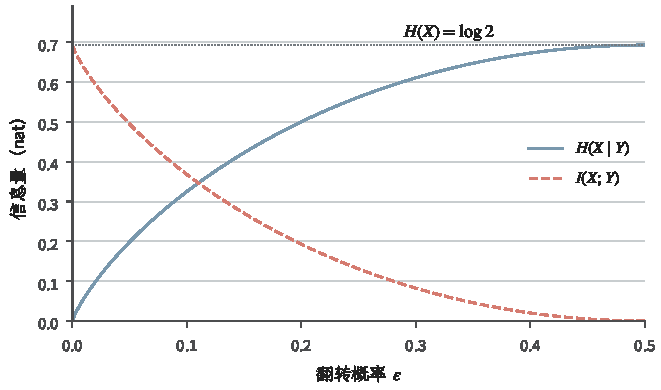
\includegraphics[width=\linewidth]{figures/01-mathematical-preliminaries/04-random-variables-distributions-and-causality/matplotlib/concepts-probability/information-binary-channel-information.pdf}
  \caption{公平二元输入通过独立翻转通道后的信息分配（解析式教学图）。蓝实线为剩余条件熵\(H_{\mathrm b}(\varepsilon)\)，红虚线为互信息\(\log2-H_{\mathrm b}(\varepsilon)\)，均以nat计。输入熵保持不变，零噪声与公平翻转分别对应完整信息与零信息。}
  \label{fig:information-binary-channel-information}
\end{figure}
由于对两个变量分别施加可逆变换会同时推送联合分布与边缘乘积，
互信息继承KL的不变性。这与微分熵随坐标单位改变形成区别。

\subsubsection{条件关系的互信息}
\label{sec:information-conditional-mi}

已经知道\(Z\)时，应在同一个条件值下判断\(X,Y\)是否还有关系，
再按\(Z\)的发生概率平均。不能把三者的边缘依赖随意相减。

\begin{definition}[条件互信息]
\label{def:information-conditional-mi}
设\(X,Y,Z\)取值于标准Borel空间，因而存在所需正则条件分布。
\term{条件互信息}（conditional mutual information）定义为
\begin{equation}
  I(X;Y\mid Z)
  =\int D_{\mathrm{KL}}\bigl(
    P_{XY\mid z}\Vert P_{X\mid z}\otimes P_{Y\mid z}\bigr)\,P_Z(\mathrm dz).
  \label{eq:information-conditional-mutual-information}
\end{equation}
条件核的版本只需在\(P_Z\)-几乎处处确定；被积量非负，允许结果为\(+\infty\)。
\end{definition}

在不保证正则条件分布存在的一般空间上，不能不加条件地沿用这个条件核定义。
在上述条件下，零条件互信息等价于条件联合核几乎处处等于条件边缘乘积，
也就是前章的条件独立。有限熵时可写成
\(H(X\mid Z)-H(X\mid Y,Z)\)，但非负KL积分是避免无穷相减的基本口径。

条件化并不一定使互信息变小。取独立公平二元变量\(X,Y\)，令\(Z=X\oplus Y\)。
边缘上互信息为零；固定\(Z\)后，\(X\)完全决定\(Y\)，条件互信息为\(\log2\)。
反过来，若\(X=Y=Z\)为同一个公平二元变量，无条件互信息为\(\log2\)，
条件互信息却为零。前者揭示约束，后者去掉已经知道的共享信息。

后处理和序贯观测都要用到KL的条件分解。设联合规律\(P_{AB},Q_{AB}\)
满足相应绝对连续性，条件核存在。联合密度比分解为边缘比与条件比的乘积，
取对数并用塔式性质得到
\begin{equation}
  D_{\mathrm{KL}}(P_{AB}\Vert Q_{AB})
  =D_{\mathrm{KL}}(P_A\Vert Q_A)
   +\mathbb E_{A\sim P_A}
       D_{\mathrm{KL}}(P_{B\mid A}\Vert Q_{B\mid A}).
  \label{eq:information-kl-conditional-chain}
\end{equation}
每个对数比的负部可积，故有限项相加的分解也能按非负扩展值成立；
若绝对连续性失败，对应的条件或边缘项为无限。
把\(Q_{XYZ}\)选为\(P_X\otimes P_{YZ}\)，再按\((X,Y)\)与\(Z\)分组，
第一项是\(I(X;Y)\)，条件项是
\(\mathbb E_{X,Y}D_{\mathrm{KL}}(P_{Z\mid X,Y}\Vert P_{Z\mid Y})
=I(X;Z\mid Y)\)。因此
\[
  I(X;Y,Z)=I(X;Y)+I(X;Z\mid Y).
\]
这证明了互信息链式法则，而不仅是引用熵差记号。

\begin{theorem}[数据处理不等式]
\label{thm:information-data-processing}
若标准Borel随机元素满足Markov关系\(X\to Y\to Z\)，
即\(X\perp Z\mid Y\)，则\(I(X;Z)\leq I(X;Y)\)，允许扩展值。
\end{theorem}
\begin{proof}
用两种顺序分解同一联合信息量：
\[
\begin{aligned}
  I(X;Y,Z)&=I(X;Y)+I(X;Z\mid Y)=I(X;Y),\\
  I(X;Y,Z)&=I(X;Z)+I(X;Y\mid Z)\geq I(X;Z).
\end{aligned}
\]
第一行的条件项由条件独立为零，第二行的条件项非负，合并即得。
证明只作非负项的相加和比较，不需要有限熵，也没有无穷相减。
\end{proof}

处理可以是\(Z=g(Y)\)，也可以是仅依赖\(Y\)的随机通道。
若额外随机性还与\(X\)关联，Markov前提可能不成立。
信息不增加并不保证每个任务的误差严格增加；当丢弃的内容与任务无关时可以取等号。

\subsection{分布差异的比较尺度}
\label{sec:information-distribution-discrepancies}

预测评分关心对数代价，越界报警关心事件概率，温度误差还关心数值相距多远。
这些要求未必由同一个散度直接表达。下面按允许观察的对象选择比较尺度；
它们可以重合，例如某些搬运距离也能写成测试函数的期望差。

\subsubsection{概率权重的差异}
\label{sec:information-probability-discrepancy}

报警规则由一个事件\(A\)指定。若尚未决定具体规则，可以问所有事件中，
哪一个的发生概率改变最多。

\begin{definition}[总变差距离]
\label{def:information-total-variation}
同一可测空间上概率测度的\term{总变差距离}（total variation distance, TV）为
\begin{equation}
  d_{\mathrm{TV}}(P,Q)=\sup_A|P(A)-Q(A)|,
  \label{eq:information-total-variation}
\end{equation}
其中上确界遍历全部可测事件。
\end{definition}

取共同支配测度\(\mu\)，密度为\(p,q\)。
由于\(\int(p-q)\,\mathrm d\mu=0\)，正部与负部积分相等。
任意事件上的差不超过正部积分，而\(A^\star=\{p\geq q\}\)达到该值，所以
\begin{equation}
  d_{\mathrm{TV}}(P,Q)=\tfrac12\int|p-q|\,\mathrm d\mu
   =P(A^\star)-Q(A^\star).
  \label{eq:information-tv-density}
\end{equation}
对\(|f|\leq1\)，积分的绝对值不超过\(\int|p-q|\)；
取\(f=2\mathbb I_{A^\star}-1\)达到上界，故
\begin{equation}
  2d_{\mathrm{TV}}(P,Q)
   =\sup_{\|f\|_\infty\leq1}|\mathbb E_Pf-\mathbb E_Qf|.
  \label{eq:information-tv-dual}
\end{equation}
若\(0\leq f\leq1\)，令\(g=2f-1\)，相应上确界则恰为\(d_{\mathrm{TV}}\)。
事件指标给出取等号的函数。这两个常数的差别来自值域宽度，不是定义冲突。

有时需要对称地比较密度形状，又希望使用Hilbert空间的几何。
把密度开平方便得到单位\(L^2\)范数的函数。

\begin{definition}[Hellinger距离]
\label{def:information-hellinger-distance}
在共同支配测度\(\mu\)下，定义平方\term{Hellinger距离}为
\begin{equation}
  d_{\mathrm H}^2(P,Q)=\tfrac12\int(\sqrt p-\sqrt q)^2\,\mathrm d\mu
   =1-\int\sqrt{pq}\,\mathrm d\mu,
  \label{eq:information-hellinger}
\end{equation}
距离本身为其非负平方根。
\end{definition}
更换共同支配测度时，两个平方根都乘以同一密度因子的平方根，
积分换元后不变。对三个分布可统一使用其和作支配测度，
从\(L^2\)三角不等式得到\(d_{\mathrm H}\)的三角不等式。
利用
\(|p-q|=|\sqrt p-\sqrt q|(\sqrt p+\sqrt q)\)，有
\[
  d_{\mathrm H}^2(P,Q)\leq d_{\mathrm{TV}}(P,Q)
  \leq\sqrt2\,d_{\mathrm H}(P,Q).
\]
左侧用\(\sqrt p+\sqrt q\geq|\sqrt p-\sqrt q|\)；
右侧用Cauchy--Schwarz以及
\(\int(\sqrt p+\sqrt q)^2\,\mathrm d\mu\leq4\)。

\begin{theorem}[Pinsker不等式]
\label{thm:information-pinsker}
以自然对数定义KL时，
\begin{equation}
  d_{\mathrm{TV}}(P,Q)\leq
  \sqrt{\tfrac12D_{\mathrm{KL}}(P\Vert Q)}.
  \label{eq:information-pinsker}
\end{equation}
\end{theorem}
\begin{proof}
KL无限时无需证明；否则\(P\ll Q\)。令
\(A=\{\mathrm dP/\mathrm dQ\geq1\}\)、\(a=P(A)\)、\(b=Q(A)\)，
则\(a-b=d_{\mathrm{TV}}(P,Q)\)。
在\(A\)及其补集分别对密度比使用条件Jensen不等式，得到
\[
  D_{\mathrm{KL}}(P\Vert Q)\geq
  a\log\frac ab+(1-a)\log\frac{1-a}{1-b}.
\]
固定\(b\in(0,1)\)，右侧作为\(a\)的函数在\(a=b\)处值和一阶导数为零，
二阶导数为\(1/[a(1-a)]\geq4\)。Taylor积分余项给出至少\(2(a-b)^2\)。
端点通过连续延拓处理；若\(b=0\)或\(1\)，有限KL迫使相应\(a=b\)。
整理即得结论。
\end{proof}

取\(P=\operatorname{Bernoulli}(1/4)\)、\(Q=\operatorname{Bernoulli}(1/2)\)，
则
\[
  d_{\mathrm{TV}}=\tfrac14,\qquad
  d_{\mathrm H}^2\approx0.0341,\qquad
  D_{\mathrm{KL}}(P\Vert Q)\approx0.1308.
\]
Pinsker给出的上界约为\(0.2557\)。这个控制不能反用：
\(P=(1-\eta)\delta_0+\eta\delta_1\)、\(Q=\delta_0\)的总变差只有\(\eta\)，
但只要\(\eta>0\)，前向KL就无限。

KL平均对数密度比；如果要限制极端密度比给事件概率带来的放大，
则可以直接控制更高阶矩。

\begin{definition}[高于一阶的Rényi散度]
\label{def:information-renyi-divergence}
对\(\alpha>1\)及\(P\ll Q\)，\term{R\'enyi散度}定义为
\begin{equation}
  D_\alpha(P\Vert Q)
   =\frac1{\alpha-1}\log\mathbb E_Q
       \left[\left(\frac{\mathrm dP}{\mathrm dQ}\right)^\alpha\right].
  \label{eq:information-renyi-divergence}
\end{equation}
若绝对连续性失败或该阶矩无限，结果为\(+\infty\)。
\end{definition}

令\(L=\mathrm dP/\mathrm dQ\)，Jensen给出
\(\mathbb E_Q L^\alpha\geq(\mathbb E_QL)^\alpha=1\)，故散度非负。
为了比较不同阶数，需要把定理~\ref{thm:linear-algebra-holder}的有限坐标配对
推广到函数积分。若\(1\leq p,q\leq\infty\)、\(1/p+1/q=1\)，且相应范数有限，则
\begin{equation}
 \int|uv|\,\mathrm d\mu\leq
 \|u\|_{L^p(\mu)}\|v\|_{L^q(\mu)}.
 \label{eq:information-integral-holder}
\end{equation}
这就是积分形式的Hölder不等式。对\(1<p,q<\infty\)，当两个范数非零时，
将\(|u|\)、\(|v|\)分别除以自己的范数，再逐点使用上述定理证明中的Young不等式并积分；
右侧归一化后为\(1/p+1/q=1\)，恢复尺度即得本式。
范数为零时相应函数几乎处处为零；端点\(p=1,q=\infty\)直接用
\(|v|\leq\|v\|_{L^\infty}\)几乎处处成立，另一端点交换两者。

取有限矩对应的\(a,b\geq1\)与\(0<t<1\)，对
\(u=L^{ta}\)、\(v=L^{(1-t)b}\)使用指数\(p=1/t\)、\(q=1/(1-t)\)，得到
\[
 \mathbb E_Q L^{ta+(1-t)b}
 \leq(\mathbb E_Q L^a)^t(\mathbb E_Q L^b)^{1-t}.
\]
取对数便说明\(K(\alpha)=\log\mathbb E_QL^\alpha\)在有限区间上为凸函数；
连同无穷值约定，它是扩展实值凸函数。
又因\(K(1)=0\)，割线斜率\(K(\alpha)/(\alpha-1)\)随阶数不减。
若某个\(\alpha_0>1\)的阶矩有限，则从右侧趋于一时可对矩函数求导，
得到\(D_\alpha\to\mathbb E_Q L\log L=D_{\mathrm{KL}}\)。
更大的阶数更强调大密度比，而不是更大的空间位移。
对上述Bernoulli例，\(\mathbb E_QL^2=1.25\)，
所以\(D_2=\log1.25\approx0.2231\)，高于KL。
事件迁移将在第~\ref{sec:information-bounded-evaluation}节使用这一阶矩；
重复机制的组合需要另外检查独立性或条件界。

\subsubsection{测试函数的期望差异}
\label{sec:information-test-functions}

如果任务只计算指定的一类函数，控制所有可测事件可能超出需要。
可以把每个允许的测试函数当作一种观测，再比较它在两个分布下的平均读数。

\begin{definition}[积分概率度量]
\label{def:information-ipm}
给定非空实值可测函数类\(\mathcal F\)，并假设每个成员在\(P,Q\)下可积，
相应的\term{积分概率度量}（integral probability metric, IPM）为
\begin{equation}
  d_{\mathcal F}(P,Q)=\sup_{f\in\mathcal F}
           |\mathbb E_Pf-\mathbb E_Qf|.
  \label{eq:information-ipm}
\end{equation}
\end{definition}
它对称并满足三角不等式，但可能为无限；如果函数类不能区分分布，
零值也可能对应不同分布，因而只给出伪距离。
选择\(\|f\|_\infty\leq1\)得到两倍TV。
选择核空间的单位球，则把比较限制为该核能够表示的函数。

\begin{definition}[最大均值差异]
\label{def:information-mmd}
设\(\mathcal H\)为再生核Hilbert空间，核\(k\)可测，且
\[
  \mathbb E_P\sqrt{k(X,X)}<\infty,\qquad
  \mathbb E_Q\sqrt{k(Y,Y)}<\infty.
\]
\term{最大均值差异}（maximum mean discrepancy, MMD）定义为
\[
  \operatorname{MMD}(P,Q)=
   \sup_{\|f\|_{\mathcal H}\leq1}|\mathbb E_Pf-\mathbb E_Qf|.
\]
\end{definition}

第~\ref{chap:functional-analysis-and-approximation}章的再生性质给出
\(|f(x)|\leq\|f\|_{\mathcal H}\sqrt{k(x,x)}\)，
所以\(f\mapsto\mathbb E_Pf\)是有界线性泛函。
Riesz表示定理保证存在唯一代表元\(\bm\mu_P\in\mathcal H\)，使
\(\mathbb E_Pf=\langle f,\bm\mu_P\rangle_{\mathcal H}\)。
这就是核均值（kernel mean embedding）：一张分布对全部核函数的平均作用。
不必预先假定Hilbert值积分存在；记号\(\mathbb E_Pk(X,\cdot)\)可由这个代表元解释。
对\(Q\)同理，于是
\[
  \operatorname{MMD}(P,Q)
  =\sup_{\|f\|_{\mathcal H}\leq1}
     |\langle f,\bm\mu_P-\bm\mu_Q\rangle|
  =\|\bm\mu_P-\bm\mu_Q\|_{\mathcal H}.
\]
差非零时取其归一化方向达到上确界。对可测有界核，所需可积条件自动满足。

\begin{definition}[核的特征性]
\label{def:information-characteristic-kernel}
在核均值均存在的指定分布类\(\mathcal P\)上，若
\(\bm\mu_P=\bm\mu_Q\)蕴含\(P=Q\)，即核均值映射为单射，
则称核\(k\)在\(\mathcal P\)上具有特征性（characteristic）。
\end{definition}

零MMD能否推出同分布，取决于这个条件。取同一对分布
\(P=\delta_0\)、\(Q=(\delta_{-1}+\delta_1)/2\)。
线性核\(k(x,y)=xy\)只比较普通均值，故MMD为零，
但\(P(\{0\})=1\)、\(Q(\{0\})=0\)。
改用高斯核\(k(x,y)=e^{-(x-y)^2/2}\)，展开核均值范数并用独立副本可得
\[
\begin{aligned}
  \operatorname{MMD}^2(P,Q)
  &=\mathbb E_{P\otimes P}k+\mathbb E_{Q\otimes Q}k
      -2\mathbb E_{P\otimes Q}k\\
  &=\tfrac32+\tfrac12e^{-2}-2e^{-1/2}>0.
\end{aligned}
\]
矩条件通过\(|k(x,y)|\leq\sqrt{k(x,x)k(y,y)}\)保证展开中的积分可交换。
图~\ref{fig:information-kernel-distinguishability}固定这两个分布，只改变核。
该算例证明高斯核能区分这一对对象，不代替整个分布类上的特征性证明。
\begin{figure*}[htbp]
  \centering
  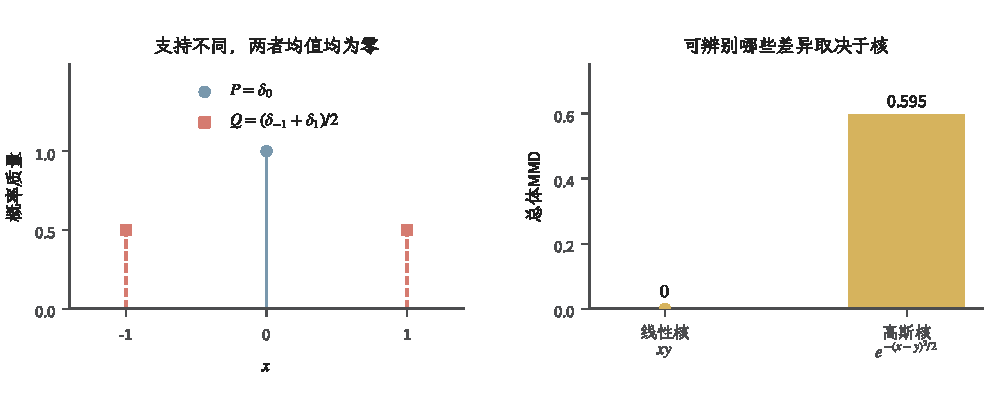
\includegraphics[width=\linewidth]{figures/01-mathematical-preliminaries/04-random-variables-distributions-and-causality/matplotlib/teaching-linear-probability/information-kernel-distinguishability.pdf}
  \caption{同均值分布在不同核下的MMD（解析式教学图）。左图为\(P=\delta_0\)与\(Q=(\delta_{-1}+\delta_1)/2\)，右图按精确总体期望计算：线性核给出零，高斯核给出约\(0.595\)。没有使用有限样本估计；差别来自测试函数类。}
  \label{fig:information-kernel-distinguishability}
\end{figure*}

\subsubsection{质量位置的搬运差异}
\label{sec:information-optimal-transport}

相邻两个点质量完全不重叠，TV已达到一，KL无限；但若结果只是温度读数，
把全部质量移动\(0.01\)度仍应属于小变化。
需要把样本空间的位置关系纳入比较。\term{最优传输}
（optimal transport, OT）寻找保持两边概率不变的最便宜配对
\scite{math-villani2009transport}

\begin{definition}[耦合]
\label{def:information-coupling}
给定\((\mathcal X,\mathcal A)\)、\((\mathcal Y,\mathcal B)\)上的概率测度\(P,Q\)，
其\term{耦合}（coupling）是乘积空间上的概率测度\(\gamma\)，满足
\[
  \gamma(A\times\mathcal Y)=P(A),\qquad
  \gamma(\mathcal X\times B)=Q(B).
\]
全体耦合记为\(\Pi(P,Q)\)。
\end{definition}
耦合规定一单位来源质量与哪部分目标质量配对，不改变两边总量。
独立耦合\(P\otimes Q\)总存在，但不一定便宜。
给定非负可测成本\(c(x,y)\)，Kantorovich搬运代价为
\begin{equation}
  \mathcal T_c(P,Q)=\inf_{\gamma\in\Pi(P,Q)}
                      \int c(x,y)\,\mathrm d\gamma(x,y).
  \label{eq:information-kantorovich-transport}
\end{equation}
下确界能否达到及怎样求解留到第~\ref{sec:information-coupling-optimization}节。
这里先把搬运用于比较分布。

\begin{definition}[Wasserstein距离]
\label{def:information-wasserstein-distance}
设\((\mathcal X,d)\)为完备可分度量空间，
\(1\leq r<\infty\)，固定基点\(x_0\)并令
\[
  \mathcal P_r(\mathcal X)=
   \left\{P:\int d(x,x_0)^r\,\mathrm dP(x)<\infty\right\}.
\]
对\(P,Q\in\mathcal P_r(\mathcal X)\)，定义
\begin{equation}
  W_r(P,Q)=\left[
    \inf_{\gamma\in\Pi(P,Q)}\int d(x,y)^r\,\mathrm d\gamma(x,y)
  \right]^{1/r}.
  \label{eq:information-wasserstein-distance}
\end{equation}
\end{definition}

由\(d(x,x_1)^r\leq2^{r-1}\{d(x,x_0)^r+d(x_0,x_1)^r\}\)，
矩条件不依赖基点；同一不等式说明独立耦合的成本有限。
对称性来自底层距离，对角耦合给出\(W_r(P,P)=0\)。
若\(W_r(P,Q)=0\)，任意有界\(L\)-Lipschitz函数的期望差至多
\(L(\mathbb E_\gamma d(X,Y)^r)^{1/r}\)，沿近最优耦合趋于零。
用连续函数\(\max\{1-kd(x,C),0\}\)逼近闭集\(C\)的指标，得到所有闭集上
\(P(C)=Q(C)\)，故\(P=Q\)。

三角不等式需要先控制随机距离之和。对\(u,v\in L^r(\mu)\)，这里使用Minkowski不等式
\(\|u+v\|_{L^r}\leq\|u\|_{L^r}+\|v\|_{L^r}\)。
它仍沿用有限维的证明：\(r=1\)直接对绝对值三角不等式积分；
\(1<r<\infty\)时，先由
\(|u+v|^r\leq2^{r-1}(|u|^r+|v|^r)\)确认\(u+v\in L^r\)，再写
\[
 \|u+v\|_{L^r}^r
 \leq\int|u+v|^{r-1}(|u|+|v|)\,\mathrm d\mu
 \leq\|u+v\|_{L^r}^{r-1}(\|u\|_{L^r}+\|v\|_{L^r}).
\]
末步对两项分别使用式~\eqref{eq:information-integral-holder}，指数为
\(r/(r-1)\)与\(r\)。非零时约去公共幂，零时结论直接成立。

还需把两个配对接起来。把\(P,Q\)的耦合分解为
\(P(\mathrm dx\mid y)Q(\mathrm dy)\)，把\(Q,R\)的耦合分解为
\(Q(\mathrm dy)R(\mathrm dz\mid y)\)。Polish空间上的正则条件分布允许构造
\[
  P(\mathrm dx\mid y)Q(\mathrm dy)R(\mathrm dz\mid y),
\]
其相邻边缘正是原来的两张耦合。这是粘合引理在这里的具体实现。
由\(d(X,Z)\leq d(X,Y)+d(Y,Z)\)及Minkowski不等式，
\[
  \bigl(\mathbb E d(X,Z)^r\bigr)^{1/r}
  \leq\bigl(\mathbb E d(X,Y)^r\bigr)^{1/r}
       +\bigl(\mathbb E d(Y,Z)^r\bigr)^{1/r}.
\]
分别选近最优耦合并令误差趋零，就得到\(W_r(P,R)\leq W_r(P,Q)+W_r(Q,R)\)。
一般成本\(c\)不具备这些距离性质，\(\mathcal T_c\)不能自动称为距离；
超出矩条件时，扩展定义还可能为无限。

对有限一阶矩的\(P,Q\)，Kantorovich--Rubinstein对偶给出
\begin{equation}
  W_1(P,Q)=\sup_{\operatorname{Lip}(f)\leq1}
                         |\mathbb E_Pf-\mathbb E_Qf|.
  \label{eq:information-kr-duality}
\end{equation}
其中\(\operatorname{Lip}(f)\leq1\)表示\(|f(x)-f(y)|\leq d(x,y)\)。
可以固定\(f(x_0)=0\)，不改变期望差，且一阶矩保证可积。
任意耦合都给出右侧不超过左侧；反向是最优传输对偶定理的实质内容，
这里按上述Polish及矩条件使用。有限空间的完整线性规划对偶将在后文推导。
这说明\(W_1\)也是IPM；\(r>1\)的\(W_r\)没有这里同一个Lipschitz单位球表达。

用同方差高斯来比较三种尺度。令\(P=\mathcal N(\mu,\sigma^2)\)、
\(Q=\mathcal N(\nu,\sigma^2)\)。取\(Y=X+\nu-\mu\)得到恒定位移耦合，
而任意耦合满足
\(\mathbb E|X-Y|^2\geq|\mathbb EX-\mathbb EY|^2=|\mu-\nu|^2\)，故
\begin{equation}
  W_2(P,Q)=|\mu-\nu|.
  \label{eq:information-gaussian-location-wasserstein}
\end{equation}
若\(\mu<\nu\)，两密度在\(c=(\mu+\nu)/2\)相交，
\(P\)在\((-\infty,c]\)上的密度较大。因此
\[
  d_{\mathrm{TV}}(P,Q)
  =P((-\infty,c])-Q((-\infty,c])
  =2\Phi\left(\frac{|\mu-\nu|}{2\sigma}\right)-1.
\]
当\(|\mu-\nu|=0.2,\sigma=1\)时，\(W_2=0.2\)、KL为\(0.02\)、
TV约为\(0.0797\)。若标准差\(\sigma\)减半，搬运位移不变，KL增为\(0.08\)，TV也增大。
位置差与可辨别程度因此不能互换。

图~\ref{fig:information-gaussian-distances}保留同一位置族的三尺度对照，
面板纵轴不同，不能按曲线高度判断哪一种概念更强。
\begin{figure*}[htbp]
  \centering
  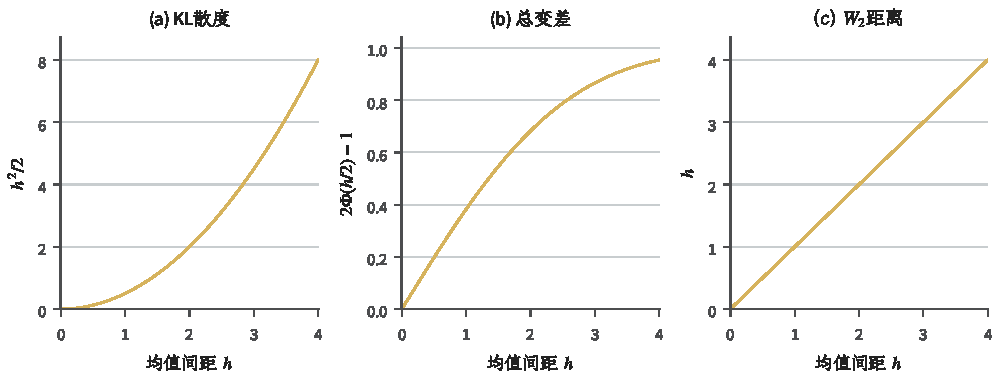
\includegraphics[width=\linewidth]{figures/01-mathematical-preliminaries/04-random-variables-distributions-and-causality/matplotlib/probability-discrete/information-gaussian-distances.pdf}
  \caption{同方差高斯位置族的解析式比较。固定\(P=\mathcal N(0,1)\)、\(Q=\mathcal N(h,1)\)，三图分别为\(D_{\mathrm{KL}}=h^2/2\)、\(d_{\mathrm{TV}}=2\Phi(h/2)-1\)与\(W_2=h\)，图中\(h\geq0\)。纵轴分别表达对数代价、事件概率差与搬运位移。}
  \label{fig:information-gaussian-distances}
\end{figure*}

对点质量\(\delta_0,\delta_\varepsilon\)，只要\(\varepsilon\neq0\)，
TV恒为一、两个方向KL均无限，而\(W_r=|\varepsilon|\to0\)。
这是支持移动在不同尺度下的极限差别。
对时间边缘分布\((P_t)\)也可比较这些距离，但它们不决定轨迹机制：
每时刻都为同一公平二元分布，既可能来自反复独立抽样，也可能来自把初次抽样永远复制。
两过程边缘距离为零，时间依赖却完全不同，必须比较联合轨迹。
实际估计MMD或Wasserstein还需考虑核、底层成本、矩和样本量；
高维经验搬运的估计误差可能很大，精确总体公式不自动给出便宜的样本估计。

\subsection{观测分布的可区分性}
\label{sec:information-lower-bounds}

分布差异也能说明推断的限度。若两个环境几乎产生相同观测，却要求不同答案，
任何程序都不能同时在两者上准确。这里固定所要恢复的目标和观测制度，
对所有估计程序给出下界；程序是否易于计算是另一问题。

\subsubsection{固定观测下的区分限制}
\label{sec:information-fixed-observations}

先把整批观测的分布视为已给定，不让程序根据中途结果改变取样位置。
两候选比较利用TV，多候选比较则需要把候选数量也纳入信息预算。

\paragraph{两个候选的区分下界}
\label{sec:information-two-candidates}

设观测\(Z\)来自\(P_0\)或\(P_1\)，先验各为\(1/2\)。
检验\(\psi(Z)\in\{0,1\}\)以事件\(A=\{\psi=1\}\)选择第二个候选，则错误和为
\[
  P_0(A)+P_1(A^{\mathsf c})=1-\{P_1(A)-P_0(A)\}.
\]
取使密度差为正的事件达到上确界，得到
\begin{equation}
  \inf_\psi\{P_0(\psi=1)+P_1(\psi=0)\}
     =1-d_{\mathrm{TV}}(P_0,P_1).
  \label{eq:information-binary-testing-tv}
\end{equation}
随机化检验只是把指标改为\([0,1]\)值函数，按TV的函数表达也不能降低这个值。
在等先验下，最小总体错误是右侧的一半；两类条件错误之和本身不是总体错误。

数值估计可以转成检验：若估计足够准，就应能知道它靠近哪个候选目标。

\begin{theorem}[Le Cam两点下界]
\label{thm:information-le-cam}
设观测模型\(P_0,P_1\)对应目标\(\theta_0,\theta_1\)，
在目标空间度量\(d\)下有\(d(\theta_0,\theta_1)\geq2s\)，\(s>0\)。
任意估计量\(\widehat\theta\)均满足
\begin{equation}
  \max_{j\in\{0,1\}}P_j\{d(\widehat\theta,\theta_j)\geq s\}
  \geq\frac{1-d_{\mathrm{TV}}(P_0,P_1)}2.
  \label{eq:information-le-cam}
\end{equation}
\end{theorem}
\begin{proof}
构造最近目标检验
\(\psi=\mathbb I\{d(\widehat\theta,\theta_1)<d(\widehat\theta,\theta_0)\}\)，
距离相等时选\(0\)。若真实为\(0\)且估计误差小于\(s\)，由三角不等式，
估计与\(\theta_1\)的距离大于\(s\)，检验不会错。
真实为\(1\)时同理。因此检验错误分别包含在估计坏事件内。
两个坏事件概率之和至少为\(1-d_{\mathrm{TV}}(P_0,P_1)\)，
其中最大者至少为一半，即得结论。
\end{proof}

若每个候选下都得到\(n\)个独立同分布观测，联合密度比是单次密度比的乘积，
取对数并平均得到
\(D_{\mathrm{KL}}(P_0^{\otimes n}\Vert P_1^{\otimes n})
=nD_{\mathrm{KL}}(P_0\Vert P_1)\)。
取单次规律为\(\mathcal N(-a,\sigma^2)\)与\(\mathcal N(a,\sigma^2)\)，
目标均值相距\(2a\)，整批KL为\(2na^2/\sigma^2\)。
令\(a=\sigma/(2\sqrt n)\)，KL为\(1/2\)，Pinsker给出TV至多\(1/2\)。
所以任何均值估计量都至少在一个候选下，以不小于\(1/4\)的概率产生
不小于\(\sigma/(2\sqrt n)\)的绝对误差。
若评价平方误差，还可由这个事件下界得到最坏风险至少\(\sigma^2/(16n)\)。
这些常数来自所选两点及放缩，不声称最优。

\paragraph{多个候选的区分下界}
\label{sec:information-many-candidates}

两点只要求区分一个二元选择；高维问题可能同时包含许多不同目标。
令\(V\)在\(\{1,\ldots,M\}\)上均匀，给定\(V=v\)后观测\(Z\sim P_v\)。
解码器\(\widehat V(Z)\)的错误概率记为\(p_{\mathrm e}\)。
即使\(Z\)连续，\(V\)的条件熵仍可按其有限后验概率求熵，再对\(Z\)积分。

\begin{theorem}[Fano不等式]
\label{thm:information-fano}
对\(M\geq2\)及上述观测模型，
\begin{equation}
  p_{\mathrm e}\geq1-\frac{I(V;Z)+\log2}{\log M}.
  \label{eq:information-fano}
\end{equation}
\end{theorem}
\begin{proof}
令\(E=\mathbb I\{\widehat V\neq V\}\)。给定\(Z\)且\(E=0\)时，
\(V=\widehat V(Z)\)已确定；给定\(E=1\)时，至多还有\(M-1\)个可能索引。
有限字母表上最大熵为均匀熵，这也可由与均匀分布的Gibbs不等式得到。
于是
\[
\begin{aligned}
  H(V\mid Z)
  &\leq H(V,E\mid Z)\\
  &=H(E\mid Z)+H(V\mid E,Z)\\
  &\leq\log2+p_{\mathrm e}\log(M-1)
   \leq\log2+p_{\mathrm e}\log M.
\end{aligned}
\]
又因\(H(V)=\log M\)，互信息分解给出
\(H(V\mid Z)=\log M-I(V;Z)\)。移项得到结论。
随机化解码可把独立随机种子并入\(Z\)，不会增加关于\(V\)的信息。
\end{proof}

若目标集合中有两两距离至少\(2s\)的有限分离集
\(\{\theta_1,\ldots,\theta_M\}\)，误差小于\(s\)就能最近邻解码。
这把前面计数与打包的工具接到统计下界：候选多能提高\(\log M\)，
但必须同时控制观测中含有多少索引信息\scite{math-cover2006information}
令\(\overline P=M^{-1}\sum_uP_u\)，则
\[
  I(V;Z)=\frac1M\sum_vD_{\mathrm{KL}}(P_v\Vert\overline P)
  \leq\frac1{M^2}\sum_{v,u}D_{\mathrm{KL}}(P_v\Vert P_u).
\]
等式来自给定\(V\)的条件KL分解；不等式来自
\(-\log(M^{-1}\sum_u p_u)\leq M^{-1}\sum_u(-\log p_u)\)。
因此
\(\max_vP_v\{d(\widehat\theta,\theta_v)\geq s\}\)
至少为Fano右侧，若右侧为负则只得到平凡下界零。

保留一个可复算的四候选构造：均值为\(\{-3a,-a,a,3a\}\)，
每个候选产生\(n\)个方差\(\sigma^2\)的独立高斯观测。
最小间距为\(2a\)，有序候选对的平均平方距离为\(10a^2\)，故
\[
  I(V;Z)\leq\frac{5na^2}{\sigma^2}.
\]
取\(a=\sigma/(4\sqrt n)\)时右侧为\(5/16\)，Fano给出
\(p_{\mathrm e}\geq1-(5/16+\log2)/\log4\approx0.2746\)。
任意估计器因此至少在一个候选上以这一概率产生不小于\(a\)的误差。
目标分离与观测接近必须同时成立；只罗列许多模型不构成下界证明。

\subsubsection{序贯观测下的区分限制}
\label{sec:information-sequential-observations}

若观测位置根据已获得的结果改变，最终资料的联合分布也随算法改变。
仍可使用前面的检验不等式，但比较对象应当是包含行动与结果的完整轨迹。

\paragraph{重复与时序观测的信息累积}
\label{sec:information-sequential-accumulation}

独立重复是简单情形。设对应分量满足绝对连续性，密度比为\(L_t\)。
乘积规律的比值为\(\prod_tL_t\)，因此
\[
\begin{aligned}
  D_{\mathrm{KL}}\left(\bigotimes_tP_t\Big\Vert\bigotimes_tQ_t\right)
     &=\sum_tD_{\mathrm{KL}}(P_t\Vert Q_t),\\
  D_\alpha\left(\bigotimes_tP_t\Big\Vert\bigotimes_tQ_t\right)
     &=\sum_tD_\alpha(P_t\Vert Q_t),\qquad\alpha>1.
\end{aligned}
\]
第一式由对数把乘积化为和；第二式由独立性使
\(\mathbb E_{\otimes Q_t}\prod_tL_t^\alpha=\prod_t\mathbb E_{Q_t}L_t^\alpha\)。
公式可按扩展值理解，不通过相减处理无限项。

一般序列不独立。设\(Z_{0:T}\)在标准Borel空间取值，两个规律分解为初始分布及
历史条件核，\(P_0\ll Q_0\)，且在相关的\(P\)-历史上
\(P_t(\cdot\mid Z_{<t})\ll Q_t(\cdot\mid Z_{<t})\)。
前章条件换测度给出联合密度比
\[
  L_{0:T}=L_0(Z_0)\prod_{t=1}^T L_t(Z_t\mid Z_{<t}).
\]
对数相加，再对每一项先按历史条件平均，得到
\begin{equation}
\begin{aligned}
 D_{\mathrm{KL}}(P_{0:T}\Vert Q_{0:T})
 &=D_{\mathrm{KL}}(P_0\Vert Q_0)\\
 &\quad+\sum_{t=1}^T\mathbb E_{Z_{<t}\sim P}
 D_{\mathrm{KL}}\bigl(P_t(\cdot\mid Z_{<t})
                     \Vert Q_t(\cdot\mid Z_{<t})\bigr).
\end{aligned}
\label{eq:information-trajectory-kl-chain}
\end{equation}
这是式~\eqref{eq:information-kl-conditional-chain}的反复应用。
有限时域中每个条件对数比的负部积分均有统一有限界，
故可合法按扩展值累加；得到有限数值则还需累计条件KL有限。
期望必须沿前向分布\(P\)实际产生的历史计算。

轨迹包含行动时，同一算法在同一历史上使用相同的条件行动核，
所以比较两个环境时行动因子相消；两个环境的历史频率却不会相消。
在同一环境比较两条策略时，则是环境核相消，剩下条件行动KL。
若两者都改变，不能省略其中任何一组项。

Rényi不能把条件散度直接按\(P\)平均。一个充分组合条件是，对每个相关历史都有
确定的统一界
\[
  D_\alpha(P_t(\cdot\mid h_{<t})\Vert Q_t(\cdot\mid h_{<t}))
  \leq\varepsilon_t.
\]
为简化记号从\(t=1\)开始且初始历史固定。在\(Q\)下从最后一步取条件期望，
\[
  \mathbb E_Q[L_t^\alpha\mid h_{<t}]
       \leq e^{(\alpha-1)\varepsilon_t}.
\]
前面的密度比是历史可测量，因此每消去一步至多乘上这个常数。
反复迭代后
\[
  \mathbb E_Q L_{1:T}^{\alpha}
  \leq e^{(\alpha-1)\sum_t\varepsilon_t},\qquad
  D_\alpha(P_{1:T}\Vert Q_{1:T})\leq\sum_t\varepsilon_t.
\]
若只在某种历史分布下给出平均条件界，后续选择可能偏向高散度历史，
不能据此使用这个组合结论。

固定有限时域无需停止论证。若共同停止规则给出\(\tau\leq T\)，
停止后补同一个吸收符号，其条件信息代价为零，公式仍适用。
无界停时则应确认在所比较的规律下几乎处处终止；
一种足够的取极限条件是截断累计对数似然比
\(\log L_{0:\tau\wedge n}\)在\(P\)下均匀可积并收敛到停止轨迹的对数密度比。
此时左侧期望可取极限，右侧的非负条件KL用单调收敛。
终止本身不能代替这些可积条件。
隐私分析若使用组合式，还必须另外规定相邻输入、随机机制，
以及对全部相邻输入统一成立的界；单个分布对的散度不是完整隐私定义。

\paragraph{自适应观测的区分下界}
\label{sec:information-adaptive-lower-bounds}

设算法\(\mathcal A\)在时刻\(t\)根据历史选择来源或状态行动对\((s,a)\)，
观测核在环境\(j\)中为\(P_j(\cdot\mid s,a)\)。
若初始规律相同、条件行动规则相同，且观测在给定历史及当前\((s,a)\)后使用该核，
轨迹链式法则可按访问位置分组：
\[
  D_{\mathrm{KL}}(\mathbb P_0^{\mathcal A}\Vert\mathbb P_1^{\mathcal A})
  =\sum_{s,a}\mathbb E_0N_T(s,a)\,
      D_{\mathrm{KL}}(P_0(\cdot\mid s,a)\Vert P_1(\cdot\mid s,a)).
\]
这里\(N_T(s,a)\)为\(T\)步中的访问次数；等式来自
\(\sum_t\mathbb I\{(S_t,A_t)=(s,a)\}=N_T(s,a)\)。
它是由算法和环境共同产生的随机量，不能预先替换成均匀独立的样本数。
核若还依赖其他历史，保留逐步条件KL形式，不能强行按固定位置常数提取。

考虑两个可选Bernoulli来源\(A,B\)。环境\(0\)的均值为
\((1/2+\varepsilon,1/2)\)，环境\(1\)为
\((1/2+\varepsilon,1/2+2\varepsilon)\)，\(0<\varepsilon<1/4\)。
每次访问给出独立于过去的相应来源新观测，但来源选择允许自适应。
两个环境的最优来源相反，全部区分信息只来自\(B\)，单次KL为
\[
  \kappa(\varepsilon)
  =D_{\mathrm{KL}}\bigl(\operatorname{Bernoulli}(1/2)
             \Vert\operatorname{Bernoulli}(1/2+2\varepsilon)\bigr)
  =-\tfrac12\log(1-16\varepsilon^2).
\]
故轨迹KL为\(\mathbb E_0N_T(B)\kappa(\varepsilon)\)。
若输出的来源在两个环境下的错误都不超过\(\delta<1/2\)，
检验恒等式迫使TV至少为\(1-2\delta\)，Pinsker进一步给出
\[
  \mathbb E_0N_T(B)\geq
  \frac{2(1-2\delta)^2}{\kappa(\varepsilon)}.
\]
例如\(\varepsilon=0.1,\delta=0.1\)，有
\(\kappa\approx0.08718\)，期望访问至少约\(14.68\)次。
当\(\varepsilon\)小时，\(\kappa=8\varepsilon^2+O(\varepsilon^4)\)，
因此固定错误水平需要\(\varepsilon^{-2}\)量级的区分观测。
这是信息不足的预算下界，不是某个算法已达到该预算的上界。
推广到无界停止必须满足上一段的终止和可积条件；
更具体的价值或累计决策损失还要引入相应任务定义。

\section{随机分布扰动与任务稳定性}
\label{sec:information-task-stability}

同一个预测器在两个测试总体上运行，平均损失能相差多少？这个问题固定评价规则，
只改变数据分布。如果预测器又是从当前评价样本中挑选的，问题就多了一层：
较低的样本损失可能来自选择过程，而非真实风险降低。
下面先控制固定函数的期望变化，再把样本与算法输出的依赖纳入比较。

\subsection{固定评价下的期望稳定性}
\label{sec:information-fixed-evaluation}

取值范围、输入敏感程度和尾部条件，分别提供三种可以利用的信息。
一个函数可能同时有界、Lipschitz且具有次高斯尾部，因此以下工具可以比较后择优使用，
并不是三类互斥任务。

\subsubsection{有界函数下的期望变化}
\label{sec:information-bounded-evaluation}

设固定可测损失\(f\)取值于\([0,1]\)。逐点恒等式
\(f(x)=\int_0^1\mathbb I\{f(x)>t\}\,\mathrm dt\)与Tonelli定理给出
\[
  |\mathbb E_Pf-\mathbb E_Qf|
  \leq\int_0^1|P(f>t)-Q(f>t)|\,\mathrm dt
  \leq d_{\mathrm{TV}}(P,Q).
\]
这也说明事件概率控制为何足以控制所有这一范围内的损失。
若\(a\leq f\leq b\)，对\((f-a)/(b-a)\)使用同一式子，得到
\[
  |\mathbb E_Pf-\mathbb E_Qf|
  \leq(b-a)d_{\mathrm{TV}}(P,Q).
\]
特别地，\(|f|\leq1\)时常数是\(2\)，不能把它与\(0\leq f\leq1\)混用。
取两点上的\(P=\delta_0,Q=\delta_1\)和\(f(0)=-1,f(1)=1\)，
期望差为\(2\)，已经表明这个因子不能删除。
结合Pinsker，还可用\((b-a)\sqrt{D_{\mathrm{KL}}(P\Vert Q)/2}\)控制期望差；
若KL无限，这个途径不给出有限信息，但TV界仍有效。

对罕见失败事件，除了TV的加性误差，还可以利用似然比高阶矩。
设\(P\ll Q\)、\(L=\mathrm dP/\mathrm dQ\)，并且某个\(\alpha>1\)满足
\(D_\alpha(P\Vert Q)<\infty\)。由H\"older不等式，
\[
  P(A)=\mathbb E_Q[L\mathbb I_A]
  \leq(\mathbb E_QL^\alpha)^{1/\alpha}
       (\mathbb E_Q\mathbb I_A^{\alpha/(\alpha-1)})^{(\alpha-1)/\alpha}.
\]
代入R\'enyi散度定义，得到
\begin{equation}
  P(A)\leq
  \exp\!\left\{\frac{\alpha-1}{\alpha}D_\alpha(P\Vert Q)\right\}
  Q(A)^{(\alpha-1)/\alpha}.
  \label{eq:information-renyi-event-bound}
\end{equation}
若\(Q(A)=0\)，绝对连续直接给出\(P(A)=0\)，无需计算无穷与零的乘积。
若\(Q(A)=0<P(A)\)，所需方向的绝对连续已经失败，相应散度无限。
例如\(D_2(P\Vert Q)\leq\log4\)、\(Q(A)\leq10^{-4}\)时，
上界为\(2\sqrt{10^{-4}}=0.02\)。这是从参考规律\(Q\)到目标规律\(P\)
的单向风险迁移，不保证反向同样成立。

有界性不能只在常见样本上成立。取
\(Q=\delta_0\)、\(P_\varepsilon=(1-\varepsilon)\delta_0+
\varepsilon\delta_{1/\varepsilon}\)，对无界函数\(f(x)=x\)，
TV为\(\varepsilon\)，期望差却恒为\(1\)。少量尾部质量足以破坏
只依赖TV的小误差结论，必须另外控制函数增长或分布尾部。

\subsubsection{敏感性约束下的期望变化}
\label{sec:information-sensitive-evaluation}

若损失不会因输入小幅移动而剧变，就应让这种敏感性进入界。
设\(P,Q\in\mathcal P_1(\mathcal X)\)，且
\(|f(x)-f(y)|\leq Ld(x,y)\)。由于
\(|f(x)|\leq|f(x_0)|+Ld(x,x_0)\)，两边期望均有限。
任意耦合\(\gamma\in\Pi(P,Q)\)满足
\[
  |\mathbb E_Pf-\mathbb E_Qf|
  =\left|\int(f(x)-f(y))\,\mathrm d\gamma\right|
  \leq L\int d(x,y)\,\mathrm d\gamma.
\]
对耦合取下确界便得到
\[
  |\mathbb E_Pf-\mathbb E_Qf|\leq LW_1(P,Q).
\]
这也可由式~\eqref{eq:information-kr-duality}直接读出。
界不要求函数有界，但同时使用了一阶矩和相对于所选距离的Lipschitz条件。

对\(\delta_0,\delta_\varepsilon\)，其中\(\varepsilon>0\)，
均值函数\(f(x)=x\)的变化恰为\(\varepsilon=W_1\)，
事件函数\(g(x)=\mathbb I\{x>0\}\)的变化却为\(1\)。
后者在零附近不连续，不属于统一Lipschitz类。
图~\ref{fig:information-small-shift-task}把同一质量位移对应的这两种评价分开显示；
小搬运距离确实保护平滑评价，但不能据此声称所有阈值事件都稳定。
\begin{figure}[htbp]
  \centering
  % Exact schematic: delta_0 and delta_epsilon under two fixed test functions.
\begin{tikzpicture}[
  x=1mm,y=1mm,
  every node/.style={font=\figurefont\footnotesize,text=FigureInk,inner sep=1pt,fill=none},
  axis/.style={draw=FigureStroke,line width=.55pt,->},
  guide/.style={draw=FigureGrid,line width=.5pt,dashed},
  curve/.style={draw=FigureStroke,line width=.85pt}
]
  \path[use as bounding box] (0,0) rectangle (112,48);
  \node at (27,44) {\(f(x)=x\)};
  \node at (86,44) {\(g(x)=\mathbb I\{x>0\}\)};
  \draw[axis] (6,12) -- (49,12) node[above=3pt] {\(x\)};
  \draw[axis] (10,12) -- (10,36);
  \draw[curve] (8,11) -- (46,30);
  \draw[guide] (38,12) -- (38,26);
  \fill[FigureBlue] (10,12) circle (1.1mm);
  \fill[FigureRed] (38,26) circle (1.1mm);
  \node[below=2pt] at (10,12) {\(0\)};
  \node[below=2pt] at (38,12) {\(\varepsilon\)};
  \node[text=FigureBlue,above left=2pt] at (10,12) {\(P\)};
  \node[text=FigureRed,above left=2pt] at (38,26) {\(Q\)};
  \draw[<->,FigureMuted,line width=.6pt] (44,12.6) -- (44,25.4);
  \node[right] at (44,19) {\(\varepsilon\)};
  \node at (27,2) {期望差：\(\varepsilon\)};
  \draw[axis] (64,12) -- (109,12) node[above=3pt] {\(x\)};
  \draw[draw=FigureStroke,line width=.55pt] (68,12) -- (68,30.9);
  \draw[axis] (68,33.1) -- (68,37);
  \draw[curve] (64,12) -- (68,12);
  \draw[curve] (69.1,32) -- (106,32);
  \draw[guide] (96,12) -- (96,32);
  \draw[draw=FigureStroke,fill=none,line width=.7pt] (68,32) circle (1mm);
  \fill[FigureBlue] (68,12) circle (1.1mm);
  \fill[FigureRed] (96,32) circle (1.1mm);
  \node[below=2pt] at (68,12) {\(0\)};
  \node[below=2pt] at (96,12) {\(\varepsilon\)};
  \node[left=3pt] at (68,32) {\(1\)};
  \node[text=FigureBlue,above left=2pt] at (68,12) {\(P\)};
  \node[text=FigureRed,above=3pt] at (96,32) {\(Q\)};
  \node at (86,2) {期望差：\(1\)};
\end{tikzpicture}

  \caption{同一小位移对两种固定评价的影响。取\(P=\delta_0\)、
  \(Q=\delta_\varepsilon\)、\(\varepsilon>0\)，底层距离为绝对值。
  左图的\(1\)-Lipschitz函数\(f(x)=x\)变化\(\varepsilon\)；
  右图的事件函数\(\mathbb I\{x>0\}\)变化\(1\)。横向位置仅作示意，
  结论对任意正的\(\varepsilon\)成立。}
  \label{fig:information-small-shift-task}
\end{figure}

MMD提供另一种敏感性约束。若同一损失\(f\)属于核\(k\)的RKHS
\(\mathcal H_k\)，且核均值存在，则再生性质和Cauchy--Schwarz不等式给出
\[
  |\mathbb E_Pf-\mathbb E_Qf|
  =|\langle f,\bm\mu_P-\bm\mu_Q\rangle_{\mathcal H_k}|
  \leq\|f\|_{\mathcal H_k}\operatorname{MMD}_k(P,Q).
\]
下标\(k\)显式标明这里沿用的核空间和MMD。
必须知道\(f\)属于该空间及其范数；核具有特征性只保证分离分布，
不自动给出任意任务函数的有限范数。
同样，若底层成本只比较图像亮度，而任务依赖没有计入成本的位置变化，
不能声称损失相对于该成本是Lipschitz。成本与核是任务假设的一部分。

\subsubsection{指数矩条件下的期望变化}
\label{sec:information-change-measure}

有些损失没有统一上界，也难以给出输入空间的敏感常数，
但在参考分布下可控制其尾部。第~\ref{sec:rv-change-measure}节
允许用密度比换测度；下面用KL和指数矩代替密度比的逐点控制。
证明的关键是指数倾斜：按\(e^f\)重新加权参考分布，使较大函数值获得更多质量。

\begin{theorem}[Donsker--Varadhan变分表达]
\label{thm:information-donsker-varadhan}
设\(P\ll Q\)。对每个有界可测实函数\(f\)，
\begin{equation}
  D_{\mathrm{KL}}(P\Vert Q)
  \geq\mathbb E_Pf-\log\mathbb E_Qe^f.
  \label{eq:information-dv-lower}
\end{equation}
而且在扩展实数意义下，
\begin{equation}
  D_{\mathrm{KL}}(P\Vert Q)
  =\sup_{f\ \text{有界可测}}\{\mathbb E_Pf-\log\mathbb E_Qe^f\}.
  \label{eq:information-dv-variational}
\end{equation}
\end{theorem}
\begin{proof}
给定有界\(f\)，令\(Z_f=\mathbb E_Qe^f\)，并定义
\[
  \frac{\mathrm dQ_f}{\mathrm dQ}=\frac{e^f}{Z_f}.
\]
因\(0<Z_f<\infty\)，且密度比严格正，\(Q_f\)与\(Q\)等价。
若\(D_{\mathrm{KL}}(P\Vert Q)<\infty\)，对数密度比可积，
乘法法则给出完整的倾斜恒等式
\[
\begin{aligned}
  D_{\mathrm{KL}}(P\Vert Q_f)
  &=\mathbb E_P\left[\log\frac{\mathrm dP}{\mathrm dQ}-f+\log Z_f\right]\\
  &=D_{\mathrm{KL}}(P\Vert Q)-\mathbb E_Pf+\log Z_f.
\end{aligned}
\]
左侧非负即得下界；若原KL无限，右侧有限，下界仍成立。

为证明上确界恰好等于KL，不能直接假设\(\log(\mathrm dP/\mathrm dQ)\)有界。
记\(L=\mathrm dP/\mathrm dQ\)，在\(L=0\)处令\(\log L=-\infty\)，取
\[
  f_n=\max\{-n,\min\{\log L,n\}\}.
\]
由于\(P(L=0)=0\)，且
\(\mathbb E_P(\log L)^-=\int_{\{L<1\}}-L\log L\,\mathrm dQ<\infty\)，
负部由支配收敛、正部由单调收敛可知
\(\mathbb E_Pf_n\to D_{\mathrm{KL}}(P\Vert Q)\)，允许极限无限。
另一方面，\(e^{f_n}\to L\)，且\(e^{f_n}\leq1+L\)。
在\(Q\)下支配收敛给出\(\mathbb E_Qe^{f_n}\to1\)，
故对应变分值趋向KL。结合已证上界，得到等式。
若\(\log L\)本身有界，它直接取到等号；一般只保证截断序列逼近。
\end{proof}

取两点均匀参考分布\(Q=(1/2,1/2)\)，\(f=(0,\log3)\)，则
\(Z_f=2\)、\(Q_f=(1/4,3/4)\)。此时
\(\mathbb E_{Q_f}f=(3/4)\log3\)，
\(D_{\mathrm{KL}}(Q_f\Vert Q)=(3/4)\log3-\log2\)，
两者之差正是\(\log Z_f\)。
这次倾斜只改变概率权重，没有改变样本的取值。

现在令\(g\)允许无界。假设\(P\ll Q\)、\(g\in L^1(P)\)，并且对所选
\(\lambda>0\)有\(\mathbb E_Qe^{\lambda g}<\infty\)。
取\(g_n=\max\{-n,\min\{g,n\}\}\)，将定理用于\(\lambda g_n\)。
因\(|g_n|\leq|g|\)、\(e^{\lambda g_n}\leq1+e^{\lambda g}\)，
分别在\(P,Q\)下支配收敛，得到
\begin{equation}
  \mathbb E_Pg
  \leq\frac{D_{\mathrm{KL}}(P\Vert Q)+\log\mathbb E_Qe^{\lambda g}}{\lambda}.
  \label{eq:information-change-measure-expectation}
\end{equation}
KL有限才能让这个界提供有限的控制。
若还知道\(g\in L^1(Q)\)，且在\(Q\)下对所有\(t\in\mathbb R\)满足
\[
  \log\mathbb E_Qe^{t(g-\mathbb E_Qg)}\leq t^2\sigma^2/2,
\]
则分别对\(g-\mathbb E_Qg\)和其相反数应用上式，得到
\[
  |\mathbb E_Pg-\mathbb E_Qg|
  \leq\frac{D_{\mathrm{KL}}(P\Vert Q)}{\lambda}+\frac{\lambda\sigma^2}{2}.
\]
当KL与\(\sigma^2\)都严格正且有限时，
取\(\lambda=\sqrt{2D_{\mathrm{KL}}(P\Vert Q)/\sigma^2}\)，得到
\begin{equation}
  |\mathbb E_Pg-\mathbb E_Qg|
  \leq\sqrt{2\sigma^2D_{\mathrm{KL}}(P\Vert Q)}.
  \label{eq:information-subgaussian-change-measure}
\end{equation}
KL为零时\(P=Q\)；\(\sigma^2=0\)时\(g\)在\(Q\)下为常量，
由绝对连续在\(P\)下也如此，所以这两个边界情形仍成立。
对\(Q=\mathcal N(0,1)\)、\(P=\mathcal N(m,1)\)、\(g(x)=x\)，
方差代理为\(1\)，KL为\(m^2/2\)，上界恰等于真实期望差\(|m|\)。
整个推导只控制两张既定分布下的期望；数据依赖的选择需要下一小节另行处理。

\subsection{数据依赖评价下的风险控制}
\label{sec:information-data-dependent-evaluation}

设\(S=(Z_1,\ldots,Z_n)\)为独立同分布样本，随机算法根据\(S\)输出\(W\)。
固定参数\(w\)时，经验损失是独立样本的平均；把它换成\(W\)以后，
参数和样本相互依赖，原先对固定参数的集中结论不能直接代入。
可以比较真实联合分布与人为解除依赖后的分布，也可以先建立覆盖全部候选的同一事件。

\subsubsection{平均评价偏差的信息控制}
\label{sec:information-mi-generalization}

设可测损失\(\ell(w,Z)\in[0,1]\)，新样本\(Z\)服从与训练样本相同的总体规律，
定义
\[
  \begin{aligned}
    R(w)&=\mathbb E_Z\ell(w,Z),&
    \widehat R_S(w)&=\frac1n\sum_{i=1}^n\ell(w,Z_i),\\
    g(S,w)&=R(w)-\widehat R_S(w).
  \end{aligned}
\]
固定\(w\)时，\(\mathbb E_Sg(S,w)=0\)。
Hoeffding引理对每个中心化损失给出指数矩，再用独立性相乘，有
\[
  \mathbb E_Se^{t g(S,w)}\leq e^{t^2/(8n)},\qquad t\in\mathbb R.
\]
界不依赖\(w\)。在边缘乘积\(Q=P_S\otimes P_W\)下再对\(w\)积分，
因此\(\mathbb E_Qg=0\)，且\(g\)的方差代理为\(1/(4n)\)。
真实评价使用联合分布\(P=P_{S,W}\)，换测度的代价正是
\[
  D_{\mathrm{KL}}(P\Vert Q)=I(S;W).
\]
若互信息有限，式~\eqref{eq:information-subgaussian-change-measure}给出
\begin{equation}
  \left|\mathbb E_{S,W}\{R(W)-\widehat R_S(W)\}\right|
  \leq\sqrt{\frac{I(S;W)}{2n}}.
  \label{eq:information-mi-generalization}
\end{equation}
无限互信息时右侧无限，不提供有效保证。
这是平均有符号泛化差的绝对值，并不是
\(\mathbb E|R(W)-\widehat R_S(W)|\)，更不是逐样本高概率界。

例如算法只能输出\(M\)种预测器，则\(I(S;W)\leq H(W)\leq\log M\)，
平均偏差至多\(\sqrt{\log M/(2n)}\)。若算法完全忽略训练样本，互信息为零，
平均有符号差也为零，但每个样本的经验风险仍会波动。
反过来，连续确定性输出可能携带无限互信息；参数维数有限本身不能保证信息有限。
这里所控制的是输出对评价样本的依赖，不能直接替换成参数个数。

\subsubsection{候选分布风险的同时控制}
\label{sec:information-pac-bayes}

若希望在看到样本后选择一张候选分布\(Q_S\)，并报告这张分布的风险，
可以先对所有候选建立共同的高概率事件。PAC--Bayes界采用见数据前
固定的先验\(P_0\)作为参考，惩罚候选分布偏离它的KL。
这里的“先验”和“候选分布”是风险分析对象，不要求来自贝叶斯生成模型。

\begin{theorem}[固定参数的基础PAC--Bayes界]
\label{thm:information-pac-bayes-basic}
在上述独立同分布样本和\([0,1]\)损失设定下，令\(P_0\)在观察\(S\)前固定，
且与\(S\)独立。对任意预先固定的\(\lambda>0\)与\(0<\delta<1\)，
以至少\(1-\delta\)的概率，同时对所有\(Q\ll P_0\)有
\begin{equation}
  \mathbb E_QR(\theta)
  \leq\mathbb E_Q\widehat R_S(\theta)
  +\frac{D_{\mathrm{KL}}(Q\Vert P_0)+\log(1/\delta)}{\lambda}
  +\frac{\lambda}{8n}.
  \label{eq:information-pac-bayes-basic}
\end{equation}
KL无限时将右侧解释为无限。
\end{theorem}
\begin{proof}
对每个固定\(\theta\)，Hoeffding引理给出
\(\mathbb E_Se^{\lambda(R(\theta)-\widehat R_S(\theta))}
\leq e^{\lambda^2/(8n)}\)。
先验独立于样本，Tonelli定理允许对同一个\(P_0\)平均：
\[
  \mathbb E_S\mathbb E_{\theta\sim P_0}
  e^{\lambda(R(\theta)-\widehat R_S(\theta))}
  \leq e^{\lambda^2/(8n)}.
\]
由Markov不等式，事件
\[
  \mathcal E=
  \left\{S:\mathbb E_{P_0}e^{\lambda(R-\widehat R_S)}
  \leq\frac{e^{\lambda^2/(8n)}}{\delta}\right\}
\]
满足\(P_S(\mathcal E)\geq1-\delta\)。
对任意固定在这个事件内的样本，实现后的函数
\(f(\theta)=\lambda(R(\theta)-\widehat R_S(\theta))\)有界。
对所有\(Q\ll P_0\)分别使用式~\eqref{eq:information-dv-lower}，得到
\[
  \lambda\mathbb E_Q(R-\widehat R_S)
  \leq D_{\mathrm{KL}}(Q\Vert P_0)
       +\log\mathbb E_{P_0}e^{\lambda(R-\widehat R_S)}
  \leq D_{\mathrm{KL}}(Q\Vert P_0)
       +\frac{\lambda^2}{8n}+\log(1/\delta).
\]
除以\(\lambda\)即得所需结论。事件只包含先验积分，不随\(Q\)改变，
因此在事件发生后选择的数据依赖\(Q_S\)也被同时覆盖。
\end{proof}

若\(P_0\)均匀分布在预先指定的\(M\)个候选上，
选择其中一个候选的点质量\(Q\)具有KL为\(\log M\)，
便得到这\(M\)个预测器的统一风险控制。
若\(P_0\)为连续分布，单点候选通常不对它绝对连续，
不能仍把该点估计作为有限KL的候选代入。

“固定\(\lambda\)”是事件成立的条件。观察数据后逐个候选优化右侧的
\(\lambda\)，或根据同一评价样本重选先验，都超出了上述事件。
可以预设可数参数网格并分配失败概率后使用并集界，
也可以用独立样本确定先验，再对剩余评价样本条件化应用定理。
这些额外步骤不能省略。互信息界比较联合规律与边缘乘积，给出平均偏差；
此处比较候选分布与先验，给出同时风险界，两者复用换测度代数但不是同一个保证。

\section{随机分布空间上的优化}
\label{sec:information-variational-learning}

前面把分布当作已知比较对象；现在把它当作未知量。
可以依据收益与已知矩条件选择一张分布，也可以在可计算的候选族中逼近已有目标。
另一个任务固定两张边缘分布，只优化它们的联合配对。
这些任务都能限制到参数族中求解，但参数步长是否意味着小的分布变化，
还需要局部几何来判断。

\subsection{目标分布的选择与逼近}
\label{sec:information-target-distribution}

选择目标与逼近目标有不同的已知量。收益加正则决定新目标，矩约束给出可行集合，
近似推断则固定待逼近的后验。它们会得到相似的指数形式或KL目标，
但不能因此混用支持、归一化和最优性结论。

\subsubsection{参考分布下的收益与偏离权衡}
\label{sec:information-gibbs-optimization}

设\(P_0\)是可以采样的参考规律，\(f\)为有界可测收益。
只追求最大收益可能把质量全部集中到极少数点；
同时扣除偏离参考规律的KL，就得到下面的分布优化。
\begin{theorem}[Gibbs变分式]
\label{thm:information-gibbs-variational}
对有界可测\(f\)，
\begin{equation}
  \log\mathbb E_{P_0}e^f
  =\sup_{Q\ll P_0}\{\mathbb E_Qf-D_{\mathrm{KL}}(Q\Vert P_0)\}.
  \label{eq:information-gibbs-variational}
\end{equation}
KL无限时目标约定为\(-\infty\)，唯一最优分布为
\[
  \frac{\mathrm dQ^\star}{\mathrm dP_0}
  =\frac{e^f}{Z_f},\qquad Z_f=\mathbb E_{P_0}e^f.
\]
\end{theorem}
\begin{proof}
有界性保证\(0<Z_f<\infty\)，且\(Q^\star\)与\(P_0\)等价。
对任何有限KL的\(Q\ll P_0\)，
\[
  \log\frac{\mathrm dQ}{\mathrm dQ^\star}
  =\log\frac{\mathrm dQ}{\mathrm dP_0}-f+\log Z_f.
\]
各项在\(Q\)下可积，故倾斜恒等式给出
\[
  \mathbb E_Qf-D_{\mathrm{KL}}(Q\Vert P_0)
  =\log Z_f-D_{\mathrm{KL}}(Q\Vert Q^\star)\leq\log Z_f.
\]
无限KL候选的目标已为\(-\infty\)。对\(Q^\star\)，
\(\log(\mathrm dQ^\star/\mathrm dP_0)=f-\log Z_f\)有界，
所以自身收益与KL都有限，可以直接代入取到等号。
Gibbs不等式的等号条件说明最优分布唯一。
\end{proof}

这里优化的是分布，Donsker--Varadhan表达优化的则是测试函数；
两条变分式共用同一倾斜恒等式，却交换了固定对象和优化对象。
允许无界\(f\)时，至少需要\(0<Z_f<\infty\)才能定义\(Q^\star\)；
若还满足\(\mathbb E_{P_0}[e^f|f|]<\infty\)，
则\(f\in L^1(Q^\star)\)，最优表达中的两项都有限。
对其他候选，也须限制到\(f\in L^1(Q)\)且KL有限的定义域。

只有归一化常数有限并不够。例如在整数\(k\geq1\)上取
\(P_0(k)=C e^{-k}/k^2\)、\(f(k)=k\)，其中\(C\)归一化\(P_0\)。
则\(Z_f=C\sum_{k\geq1}k^{-2}<\infty\)，而\(Q^\star(k)\)正比于\(k^{-2}\)，
导致\(\mathbb E_{Q^\star}f=\infty\)且KL无限。
此时不能把\(Q^\star\)代入\(\infty-\infty\)。
若\(f\)为有限实值且\(Z_f<\infty\)，令
\(Z_n=\mathbb E_{P_0}[e^f\mathbb I_{\{|f|\leq n\}}]\)，在\(Z_n>0\)时取
\[
  \frac{\mathrm dQ_n}{\mathrm dP_0}
  =\frac{e^f\mathbb I_{\{|f|\leq n\}}}{Z_n}.
\]
其收益和KL有限，目标恰为\(\log Z_n\to\log Z_f\)。
因而在有限目标定义域上仍可逼近上确界，不必有可直接代入的最优分布。

对有界收益\(r\)加入温度\(\beta>0\)，令\(f=r/\beta\)，可得
\[
  \sup_{Q\ll P_0}\{\mathbb E_Qr-\beta D_{\mathrm{KL}}(Q\Vert P_0)\}
  =\beta\log\mathbb E_{P_0}e^{r/\beta},\qquad
  Q^\star\propto P_0e^{r/\beta}.
\]
较小温度更偏向高收益区域，也可能使重要性权重集中、采样方差增大。
KL正则描述相对于\(P_0\)的概率偏离；若某种失败事件必须受控，
仍需用上一节的风险迁移条件或另加约束，不能把正则项本身当成安全保证。

\subsubsection{矩约束下的最大熵选择}
\label{sec:information-maximum-entropy}

若只知道均值或协方差，没有指定收益函数，哪些分布与这些信息相容？
\term{最大熵原理}在相容分布中选择熵最大的一个。
它把“不过度集中”落实到一个明确的优化准则，不表示该分布已被观测证明为真；
参考测度和矩约束仍是建模选择。

固定参考测度\(\mu\)，要求密度\(p\)满足
\[
  \int p\,\mathrm d\mu=1,\qquad
  \int \bm T(x)p(x)\,\mathrm d\mu(x)=\bm\tau.
\]
若存在有限参数\(\bm\lambda\)，使
\[
  p_{\bm\lambda}(x)
  =\exp\{\bm\lambda^\top\bm T(x)-A(\bm\lambda)\},\qquad
  A(\bm\lambda)=\log\int e^{\bm\lambda^\top\bm T(x)}\,\mathrm d\mu(x)<\infty
\]
归一化并满足这些矩约束，则它是最大熵的候选。
形式上，对熵加归一化和矩约束的Lagrange项，密度方向的一阶条件为
\(-\log p-1+\bm\lambda^\top\bm T+a=0\)，从而给出上述指数形式。
但这一步没有证明解存在，也没有处理所有无限维变分的合法性；
真正的最优性可由KL直接核验。

对任意同样可行、统计量可积且熵有限的密度\(p\)，若候选自身也满足这些有限性条件，
\[
\begin{aligned}
  D_{\mathrm{KL}}(p\Vert p_{\bm\lambda})
  &=\int p\log p\,\mathrm d\mu-\bm\lambda^\top\bm\tau+A(\bm\lambda)\\
  &=-h_\mu(p)+h_\mu(p_{\bm\lambda})\geq0.
\end{aligned}
\]
因此候选最大化熵，等号当且仅当两密度几乎处处相同。
矩约束不可达、配分函数无限或最大熵没有上界时，乘子方程不能弥补这些缺口。
即使最大熵分布存在，边界约束也可能只能由无穷自然参数的极限表示。

固定均值\(\bm m\)和正定协方差\(\bm\Sigma\)时，
\(q=\mathcal N(\bm m,\bm\Sigma)\)给出一个完整实例。
其对数密度为
\[
  \log q(\bm x)
  =-\frac d2\log(2\pi)-\frac12\log\det\bm\Sigma
   -\frac12(\bm x-\bm m)^\top\bm\Sigma^{-1}(\bm x-\bm m).
\]
任意具有同样均值和协方差的密度\(p\)都满足
\[
  \mathbb E_p[(\bm X-\bm m)^\top\bm\Sigma^{-1}(\bm X-\bm m)]
  =\operatorname{tr}(\bm\Sigma^{-1}\bm\Sigma)=d.
\]
因而\(\mathbb E_p\log q=\mathbb E_q\log q\)，在\(h(p)\)有限时，
\[
  D_{\mathrm{KL}}(p\Vert q)=h(q)-h(p)\geq0,\qquad
  h(p)\leq\frac12\log\{(2\pi e)^d\det\bm\Sigma\}.
\]
等号唯一对应高斯。这仍是在固定坐标和Lebesgue参考测度下比较微分熵。
协方差奇异时，分布被限制在低维仿射子空间，不能继续使用原空间中的密度公式；
须改用子空间参考测度。

指数形式还把分布优化与参数表示联系起来。
对前章的指数族
\[
  p_{\bm\eta}(x)
  =h(x)\exp\{\bm\eta^\top\bm T(x)-A(\bm\eta)\},
\]
在允许交换微分积分的自然参数内部，
\(\nabla A(\bm\eta)=\mathbb E_{\bm\eta}\bm T=\bm\tau\)，
\(\nabla^2A(\bm\eta)=\operatorname{Cov}_{\bm\eta}(\bm T)\)。
自然参数\(\bm\eta\)指定指数权重，均值参数\(\bm\tau\)指定统计量平均。
回用第~\ref{chap:optimization}章的凸共轭，定义
\begin{equation}
  A^\star(\bm\tau)
  =\sup_{\bm\eta}\{\bm\eta^\top\bm\tau-A(\bm\eta)\}.
  \label{eq:information-log-partition-conjugate}
\end{equation}
若\(\bm\tau=\nabla A(\bm\eta)\)由有限自然参数实现，凸性的一阶不等式给出
\(A(\bm\zeta)\geq A(\bm\eta)+\bm\tau^\top(\bm\zeta-\bm\eta)\)。
移项可知共轭上确界在\(\bm\eta\)达到，且
\[
  A^\star(\bm\tau)=\bm\eta^\top\bm\tau-A(\bm\eta)
  =\int p_{\bm\eta}\log\frac{p_{\bm\eta}}h\,\mathrm d\mu.
\]
最后一个量是相对于基准项\(h\)的负熵；若\(h\)本身为概率密度，它就是KL。
只有\(h=1\)时才能直接写成普通负熵。

两组参数能否在局部互换，还取决于统计量有无冗余。所谓最小表示，是指不存在非零向量
\(\bm a\)，使\(\bm a^\top\bm T(x)\)在基准测度\(h\,\mathrm d\mu\)下几乎处处为常量。
在自然参数空间的开内部，这个条件给出
\[
 \bm a^\top\operatorname{Cov}_{\bm\eta}(\bm T)\bm a
 =\operatorname{Var}_{\bm\eta}(\bm a^\top\bm T)>0
 \qquad(\bm a\neq\bm0),
\]
因为有限自然参数的指数因子严格为正，模型分布与基准测度具有相同的零测集。
所以协方差正定，\(\mathrm d\bm\tau=\nabla^2A\,\mathrm d\bm\eta\)的Jacobian可逆，
由逆函数定理可得两组参数局部一一对应。
若统计量有含常量项的仿射冗余，例如某一坐标恒为\(1\)，协方差就会奇异；
只排除不同统计量之间的线性组合还不够。

有限配置可以不预设每个均值都由有限参数实现，而直接覆盖闭可行域。
\begin{theorem}[有限配置上的配分函数与最大熵对偶]
\label{thm:information-finite-entropy-duality}
设\(D\)为有限非空配置集，\(\bm T:D\to\mathbb R^m\)，基准权重恒为\(1\)。
定义
\[
  A(\bm\theta)=\log\sum_{z\in D}e^{\langle\bm\theta,\bm T(z)\rangle},
  \qquad\mathcal M=\operatorname{conv}\{\bm T(z):z\in D\}.
\]
对\(\bm\mu\in\mathcal M\)，令
\[
  H^\star(\bm\mu)=\max_{q:\,\mathbb E_q\bm T=\bm\mu}H(q),
\]
其中\(q\)遍历\(D\)上的全部概率质量函数。则在整个\(\mathcal M\)上有
\(A^\star(\bm\mu)=-H^\star(\bm\mu)\)，在外部有\(A^\star=+\infty\)，且
\begin{equation}
  A(\bm\theta)=\max_{\bm\mu\in\mathcal M}
  \{\langle\bm\theta,\bm\mu\rangle+H^\star(\bm\mu)\}.
  \label{eq:information-finite-gibbs-duality}
\end{equation}
\end{theorem}
\begin{proof}
有限概率单纯形紧；给定可行均值后的约束闭且非空，熵在单纯形上连续，
因此每个\(H^\star(\bm\mu)\)都能达到。
令\(p_{\bm\theta}(z)=e^{\langle\bm\theta,\bm T(z)\rangle-A(\bm\theta)}\)。
对任意质量函数\(q\)，展开有限KL得到
\[
  \langle\bm\theta,\mathbb E_q\bm T\rangle+H(q)
  =A(\bm\theta)-D_{\mathrm{KL}}(q\Vert p_{\bm\theta})
  \leq A(\bm\theta),
\]
且在\(q=p_{\bm\theta}\)处取等号。把所有\(q\)按均值分组，
组内线性项相同，只需保留最大熵者，即得式~\eqref{eq:information-finite-gibbs-duality}。

为证明边界处也有共轭等式，在\(\mathcal M\)上令\(f=-H^\star\)，
在外部令\(f=+\infty\)。
取两个均值及其最大熵分布\(q_1,q_2\)，混合
\(tq_1+(1-t)q_2\)的均值为对应均值的凸组合。
熵凹性给出
\[
  H^\star(t\bm\mu_1+(1-t)\bm\mu_2)
  \geq H(tq_1+(1-t)q_2)
  \geq tH^\star(\bm\mu_1)+(1-t)H^\star(\bm\mu_2).
\]
所以\(f\)凸。
若\(\bm\mu_n\to\bm\mu\)且各均值可行，先取使最大熵值趋于上极限的子列，
再从对应的最大熵分布中取收敛子列\(q_{n_k}\to q\)。
有限维均值映射连续，故\(\mathbb E_q\bm T=\bm\mu\)；熵连续性给出
\[
  \limsup_nH^\star(\bm\mu_n)=H(q)\leq H^\star(\bm\mu).
\]
于是\(H^\star\)上半连续。又因\(\mathcal M\)闭，
扩展后的\(f\)在整个\(\mathbb R^m\)上下半连续。
由\(0\leq H^\star\leq\log|D|\)和\(\mathcal M\neq\varnothing\)，
\(f\)适当。前半证明已说明\(f^\star=A\)，
定理~\ref{thm:opt-fenchel-moreau}于是给出
\(A^\star=f^{\star\star}=f\)，包括边界均值和可行域外部。
此证明不要求共轭上确界由有限自然参数达到。
\end{proof}

\(\mathcal M\)是可实现统计量均值的凸包。
统计量由各局部配置的指示函数组成时，它称为边缘多面体；
属于该集合表示局部概率表能同时来自同一全局分布，
强于每张表单独归一化。例如两个二元变量的两张边缘表均令取值\(1\)的概率为\(0.1\)，
则联合表不可能同时要求\(P(X=1,Y=1)=0.9\)。
局部数字各自在\([0,1]\)内，并不足以保证共同可实现。

在\(\{0,1,2\}\)上要求\(\mathbb EX=1/2\)时，最大熵分布为
\(p_j=t^j/(1+t+t^2)\)。均值方程给出
\[
  \frac{t+2t^2}{1+t+t^2}=\frac12,\qquad
  3t^2+t-1=0,\qquad
  t=\frac{\sqrt{13}-1}{6}\approx0.4343.
\]
故\((p_0,p_1,p_2)\approx(0.6162,0.2676,0.1162)\)。
自然参数是\(\lambda=\log t\)，
\(H(p)=\log(1+t+t^2)-\lambda/2\)，与共轭负熵一致。
若均值改为边界值\(0\)，唯一可行分布为\(\delta_0\)，熵为零；
它由\(t\downarrow0\)、\(\lambda\to-\infty\)逼近，却没有有限自然参数表示。
这正是分布最优解存在与有限参数实现之间的区别。

\subsubsection{表示约束下的目标分布逼近}
\label{sec:information-elbo-approximation}

若目标已经由联合模型确定，就不再自由选择规律，而是在可计算的候选族中逼近它。
固定观测\(x\)和模型参数\(\bm\theta\)，设
\[
  0<p_{\bm\theta}(x)=\int p_{\bm\theta}(x,z)\,\mathrm dz<\infty,
  \qquad
  \pi(z)=p_{\bm\theta}(z\mid x).
\]
记候选密度为\(q\)。证据积分可能难算，候选\(q\)则允许采样和评价密度。

\begin{definition}[证据下界]
\label{def:information-elbo}
若\(q\ll\pi\)且\(D_{\mathrm{KL}}(q\Vert\pi)<\infty\)，定义
\term{证据下界}（evidence lower bound, ELBO）为
\[
  \mathcal L(q,\bm\theta;x)
  =\mathbb E_q\log\frac{p_{\bm\theta}(x,Z)}{q(Z)}.
\]
按对数比整体取期望，不要求\(\mathbb E_q\log p_{\bm\theta}(x,Z)\)
与\(\mathbb E_q\log q(Z)\)各自有限。
\end{definition}

有限KL保证上述整体对数比可积，因为它等于
\(\log p_{\bm\theta}(x)-\log(q/\pi)\)。
直接分解就得到
\begin{equation}
  \log p_{\bm\theta}(x)
  =\mathcal L(q,\bm\theta;x)+D_{\mathrm{KL}}(q\Vert p_{\bm\theta}(\cdot\mid x)).
  \label{eq:information-elbo-decomposition}
\end{equation}
因此它确为下界，等号当且仅当\(q=\pi\)。
若KL无限，可以把ELBO扩展为\(-\infty\)，
但应使用\(\mathcal L=\log p_{\bm\theta}(x)-D_{\mathrm{KL}}\)这一方向，
不把右侧的\(-\infty+\infty\)当作合法分解。

另一条常见推导先乘除\(q\)，再使用Jensen不等式。
这里重要性等号需要相反方向的覆盖条件\(\pi\ll q\)，
保证联合密度的正质量区域不会被\(q\)漏掉。
若同时满足\(q\ll\pi\)和上述可积性，则
\begin{align}
  \log p_{\bm\theta}(x)
  &=\log\mathbb E_q\left[\frac{p_{\bm\theta}(x,Z)}{q(Z)}\right]\notag\\
  &\geq\mathbb E_q\log\frac{p_{\bm\theta}(x,Z)}{q(Z)}
   =\mathcal L(q,\bm\theta;x).
  \label{eq:information-elbo-jensen}
\end{align}
只满足\(q\ll\pi\)时，KL分解仍成立，
但重要性期望实际为\(p_{\bm\theta}(x)\pi(\{q>0\})\)，可能小于证据。
例如\(\pi=(1/2,1/2)\)、\(q=(1,0)\)，KL为\(\log2\)，
ELBO是\(\log p_{\bm\theta}(x)-\log2\)，而重要性期望只恢复一半证据。
反过来，若\(\pi=(1,0)\)、\(q=(1/2,1/2)\)，虽完整覆盖目标，
但\(q\)在零后验区域放了质量，反向KL无限。两种支持要求不能互相代替。

固定模型后最大化ELBO，等价于在候选族\(\mathcal Q\)中最小化
\(D_{\mathrm{KL}}(q\Vert\pi)\)。
若最优候选\(q^\star_{\mathcal Q}\)存在，则实际候选的KL可写为
\[
  D_{\mathrm{KL}}(q\Vert\pi)
  =\inf_{\widetilde q\in\mathcal Q}D_{\mathrm{KL}}(\widetilde q\Vert\pi)
   +\left[D_{\mathrm{KL}}(q\Vert\pi)
    -\inf_{\widetilde q\in\mathcal Q}D_{\mathrm{KL}}(\widetilde q\Vert\pi)\right].
\]
第一项是表示限制，第二项是未达到族内最优的求解误差。
即使最优候选不存在，这个按下确界的分解仍有效。
若同时拟合\(\bm\theta\)，证据和后验也随之改变，
模型与真实数据规律的拟合误差是另一层问题，不等于这两项之和。

取\(Z\sim\mathcal N(0,1)\)、\(X\mid Z\sim\mathcal N(Z,1)\)，观测\(x=1\)。
配平方得到后验\(\mathcal N(1/2,1/2)\)，证据为\(\mathcal N(0,2)\)。
若\(q=\mathcal N(0,1)\)，
\[
\begin{aligned}
  \log p(x)&=-\tfrac12\log(4\pi)-\tfrac14\approx-1.5155,\\
  D_{\mathrm{KL}}(q\Vert\pi)
  &=\tfrac12\{2+\tfrac12-1+\log(1/2)\}\approx0.4034,\\
  \mathcal L(q;x)&\approx-1.9189.
\end{aligned}
\]
三者满足精确分解。多变量情形把\(q\)限制为分块独立族，
可能留下无法表示的后验相关性；求解更充分也不能消除这一表示限制。

分布蒸馏采用另一个给定目标：教师的条件分布\(P_{\mathrm T}(\cdot\mid x)\)。
在固定输入权重下，最小化
\(D_{\mathrm{KL}}(P_{\mathrm T}\Vert Q_{\bm\phi})\)
等价于教师软标签下的交叉熵，要求学生覆盖教师的正质量类别。
反向KL改由学生平均，支持要求和最优近似都会改变。
学生逼近教师，不自动意味着更接近真实标签规律。

对比目标则改变了评价和采样机制：把一个联合配对样本与若干边缘负样本组成分类任务。
以一个具体的InfoNCE损失为例，取总候选数\(K\geq2\)，按目标联合分布抽取
\((X,Y_1)\)，再独立地按边缘\(P_Y\)抽取\(Y_2,\ldots,Y_K\)；
这些负样本彼此独立，也独立于\((X,Y_1)\)。对可测实值评分函数\(s\)，定义
\begin{equation}
 \mathcal L_K
 =\mathbb E\left[-\log
   \frac{\exp s(X,Y_1)}{\sum_{j=1}^K\exp s(X,Y_j)}\right].
 \label{eq:information-contrastive-loss}
\end{equation}
它把相对评分归一化为候选类别概率，再惩罚未能认出正样本的预测。
\(K\)包括一个正样本和\(K-1\)个负样本；期望针对上述全部抽样。
若该损失可积，则
\[
 \log K-\mathcal L_K\leq I(X;Y).
\]

这个下界可从分类熵推得。等价地，先在\(K\)个位置中均匀选正样本位置\(J\)，
令该位置与\(X\)按目标联合分布配对，其余位置仍为独立边缘样本。
记整组观测为\(W=(X,Y_1,\ldots,Y_K)\)。
同一个评分规则在各位置对称使用，所以平均分类损失仍为\(\mathcal L_K\)；
由对数损失的最优性，它不小于真实类别条件熵\(H(J\mid W)\)。因此
\[
 \log K-\mathcal L_K\leq H(J)-H(J\mid W)=I(J;W).
\]
还需说明识别正样本位置的信息不会超过目标互信息。令\(P_j\)为给定\(J=j\)的
\(W\)分布，\(M=K^{-1}\sum_jP_j\)，并以完全独立规律
\(Q=P_X\otimes P_Y^{\otimes K}\)作参照。若\(I(X;Y)<\infty\)，
每个\(P_j\)相对于\(Q\)只有正样本配对这一项密度比，所以
\[
\begin{aligned}
 I(X;Y)&=\frac1K\sum_{j=1}^KD_{\mathrm{KL}}(P_j\Vert Q)\\
 &=\frac1K\sum_{j=1}^KD_{\mathrm{KL}}(P_j\Vert M)
      +D_{\mathrm{KL}}(M\Vert Q)\\
 &=I(J;W)+D_{\mathrm{KL}}(M\Vert Q)\geq I(J;W).
\end{aligned}
\]
中间等式将对数密度比拆成经过\(M\)的两项，再对\(j\)平均；
互信息无限时原下界自动成立。
又因分类损失非负，\(\log K-\mathcal L_K\leq\log K\)，
有限候选数确实会限制这个下界的最大数值。
不符合采样假设时，不能把优化该分类目标直接解释为增加原分布的互信息；
即使下界合法，也不自动保证校准、语义质量或下游风险。

\subsection{固定边缘的耦合优化}
\label{sec:information-coupling-optimization}

现在来源分布\(P\)和目标分布\(Q\)都已固定，未知量是联合分布
\(\gamma\in\Pi(P,Q)\)。独立配对总可行，却未必便宜；
优化要在不改变行列总质量的前提下，决定哪些来源质量送往哪些目标。
定义~\ref{def:information-coupling}与式~\eqref{eq:information-kantorovich-transport}
已经给出可行集合和成本，这里补足最小值的存在与有限求解。

\subsubsection{最优耦合的存在条件}
\label{sec:information-optimal-coupling-existence}

有限表格不会丢失总质量，但一般空间中的一列近最优方案可能把质量送往越来越远处。
证明存在性，要同时防止质量逃逸、保住固定边缘，并使极限成本不增加。
第~\ref{sec:rv-weak-convergence}节的概率测度弱收敛及紧性正好服务这三步。
这里不重新定义它们：变化对象是乘积空间上的概率测度，
测试函数是有界连续函数；这不同于泛函分析中固定线性空间内由连续线性泛函
检验的弱拓扑。二者都有“弱收敛”这一中文名称，但不能不说明对象就互换结论。

\begin{theorem}[最优耦合存在]
\label{thm:information-optimal-coupling-existence}
设\(\mathcal X,\mathcal Y\)为Polish空间，\(P,Q\)为其Borel概率测度。
若成本\(c:\mathcal X\times\mathcal Y\to[0,\infty]\)下半连续，
且至少有一个\(\gamma_0\in\Pi(P,Q)\)满足\(\int c\,\mathrm d\gamma_0<\infty\)，
则存在有限成本耦合\(\gamma^\star\)达到
\(\mathcal T_c(P,Q)=\inf_{\gamma\in\Pi(P,Q)}\int c\,\mathrm d\gamma\)。
\end{theorem}
\begin{proof}
可行集合非空，且成本非负、有有限可行值，所以最优下确界有限。
取近最优序列\(\gamma_n\in\Pi(P,Q)\)，使
\(\int c\,\mathrm d\gamma_n\to\mathcal T_c(P,Q)\)。

Polish空间上的Borel概率测度紧。
任给\(\varepsilon>0\)，分别选择紧集\(K_{\mathcal X},K_{\mathcal Y}\)，使
\(P(K_{\mathcal X}^{\mathsf c})<\varepsilon/2\)、
\(Q(K_{\mathcal Y}^{\mathsf c})<\varepsilon/2\)。
其乘积紧，且任意可行耦合都满足
\[
  \gamma((K_{\mathcal X}\times K_{\mathcal Y})^{\mathsf c})
  \leq P(K_{\mathcal X}^{\mathsf c})+Q(K_{\mathcal Y}^{\mathsf c})
  <\varepsilon.
\]
因边缘固定，这个紧集对全部\(\gamma\)同时适用，
从而\((\gamma_n)\)一致紧。
乘积空间仍为Polish空间，定理~\ref{thm:rv-prokhorov}给出子列
\(\gamma_{n_k}\Rightarrow\gamma^\star\)。

对任意有界连续\(a:\mathcal X\to\mathbb R\)，函数
\((x,y)\mapsto a(x)\)有界连续，故
\[
  \int a(x)\,\mathrm d\gamma^\star(x,y)
  =\lim_k\int a(x)\,\mathrm d\gamma_{n_k}(x,y)=\int a\,\mathrm dP.
\]
有界连续函数区分Borel概率测度，因此\(\gamma^\star\)的第一边缘为\(P\)。
同理第二边缘为\(Q\)，所以极限仍可行。

最后，对非负下半连续成本使用定理~\ref{thm:rv-portmanteau}：
\[
  \int c\,\mathrm d\gamma^\star
  \leq\liminf_k\int c\,\mathrm d\gamma_{n_k}
  =\mathcal T_c(P,Q).
\]
可行性又给出反向不等式，所以等号成立且成本有限。
\end{proof}

最后一步的积分测度随\(k\)改变，不能用固定测度下的Fatou引理直接替代。
非负性避免成本的负部失控，下半连续性保证极限不会突然增加成本；
若修改这些假设，需要另给能实现同样作用的条件。
存在联合耦合也不保证存在确定搬运映射。
例如\(P=\delta_0\)、\(Q=(\delta_{-1}+\delta_1)/2\)时，
唯一来源点必须把质量分成两半，任何单值映射都只能把它送到一个点。

\subsubsection{有限空间的搬运求解}
\label{sec:information-finite-transport}

设来源点为\(x_i\)、目标点为\(y_j\)，概率向量为\(\bm p,\bm q\)，
各成本\(c_{i,j}\)有限且非负。搬运表\(\bm\gamma\)的行和是来源质量，
列和是目标质量，问题为
\[
  \min_{\gamma_{i,j}\geq0}\sum_{i,j}c_{i,j}\gamma_{i,j},
  \qquad \sum_j\gamma_{i,j}=p_i,\quad\sum_i\gamma_{i,j}=q_j.
\]
独立表\(\gamma_{i,j}=p_iq_j\)可行。
约束集合闭，且每个元素在\([0,1]\)内，因此它是紧多面体，
线性目标可以取到最小值。

回用第~\ref{chap:optimization}章线性规划，为两组边缘约束引入势函数
\(u_i,v_j\)，保留\(\gamma_{i,j}\geq0\)作为取下确界的定义域：
\begin{align}
  \mathcal L(\bm\gamma,\bm u,\bm v)
  &=\sum_{i,j}c_{i,j}\gamma_{i,j}
    +\sum_i u_i\left(p_i-\sum_j\gamma_{i,j}\right)
    +\sum_j v_j\left(q_j-\sum_i\gamma_{i,j}\right)\notag\\
  &=\sum_i u_ip_i+\sum_jv_jq_j
    +\sum_{i,j}(c_{i,j}-u_i-v_j)\gamma_{i,j}.
  \label{eq:information-discrete-ot-lagrangian}
\end{align}
如果某个系数\(c_{i,j}-u_i-v_j<0\)，将对应非负变量趋向无穷，
Lagrangian下确界就是\(-\infty\)。
若全部系数非负，下确界可在\(\bm\gamma=\bm0\)取到，
值为\(\sum_i u_ip_i+\sum_jv_jq_j\)。
这里消元时边缘等式已进入Lagrangian，不再限制\(\bm\gamma\)，
所以零表虽不是原问题的可行表，却可以用于计算对偶函数。
于是
\[
  g(\bm u,\bm v)=
  \begin{cases}
    \sum_i u_ip_i+\sum_jv_jq_j,&u_i+v_j\leq c_{i,j}\text{ 对所有 }i,j,\\
    -\infty,&\text{否则}.
  \end{cases}
\]
最大化它得到
\begin{equation}
  \max_{\bm u,\bm v}
  \left\{\sum_i u_ip_i+\sum_jv_jq_j:\ u_i+v_j\leq c_{i,j}\right\}.
  \label{eq:information-discrete-ot-dual}
\end{equation}
势函数约束来自消元后下确界有限的必要充分条件，不是额外猜出的搬运规则。
对任意原始可行表，将\(u_i+v_j\leq c_{i,j}\)逐项乘\(\gamma_{i,j}\)
并求和，立刻得到对偶值不超过搬运成本。
有限维原问题可行且最优值有限，线性规划强对偶又保证两者最优值相等。

仍取位置\(0,2\)，令\(\bm p=(3/4,1/4)\)、\(\bm q=(1/4,3/4)\)，
\(c_{i,j}=|x_i-y_j|\)。全部可行表都能写成
\[
  \bm\gamma(a)=
  \begin{pmatrix}
    a&3/4-a\\
    1/4-a&a
  \end{pmatrix},\qquad 0\leq a\leq1/4.
\]
对角线成本为零，两个非对角线成本均为\(2\)，
故总成本为\(2-4a\)，在\(a=1/4\)处最小：
\[
  \bm\gamma^\star=
  \begin{pmatrix}1/4&1/2\\0&1/4\end{pmatrix},\qquad
  \sum_{i,j}c_{i,j}\gamma^\star_{i,j}=1.
\]
对偶取\(\bm u=(0,-2)\)、\(\bm v=(0,2)\)，四项和依次为
\(0,2,-2,0\)，均不超过对应成本\(0,2,2,0\)。
对偶值为
\[
  \bm u^\top\bm p+\bm v^\top\bm q
  =-2(1/4)+2(3/4)=1.
\]
弱对偶已足以核验最优性：所有可行表成本至少为\(1\)，而上表恰好达到。
图~\ref{fig:information-transport-tables}比较这个表与独立配对，
说明相同行列边缘不能决定搬运成本。
\begin{figure}[htbp]
  \centering
  % Rows: source locations 0,2. Columns: target locations 0,2.
\begin{tikzpicture}[
  x=1mm,y=1mm,
  every node/.style={font=\figurefont\footnotesize,text=FigureInk,inner sep=1pt,fill=none},
  grid/.style={draw=FigureStroke,line width=.6pt}
]
  \path[use as bounding box] (0,0) rectangle (112,59);
  \foreach \offset/\heading in {0/独立配对,58/最优配对} {
    \begin{scope}[shift={(\offset,0)}]
      \node at (26,55) {\heading};
      \fill[FigureYellowFill] (21,29) rectangle (34,40);
      \fill[FigureYellowFill] (8,18) rectangle (21,29);
      \draw[grid] (8,18) rectangle (34,40);
      \draw[grid] (21,18) -- (21,40);
      \draw[grid] (8,29) -- (34,29);
      \node at (14.5,44) {\(0\)};
      \node at (27.5,44) {\(2\)};
      \node at (3,34.5) {\(0\)};
      \node at (3,23.5) {\(2\)};
      \node[text=FigureBlue] at (43,44) {行和};
      \node[text=FigureBlue] at (43,34.5) {\(3/4\)};
      \node[text=FigureBlue] at (43,23.5) {\(1/4\)};
      \node[text=FigureRed] at (14.5,12) {\(1/4\)};
      \node[text=FigureRed] at (27.5,12) {\(3/4\)};
      \node[text=FigureRed] at (43,12) {列和};
    \end{scope}
  }
  \node at (14.5,34.5) {\(3/16\)};
  \node at (27.5,34.5) {\(9/16\)};
  \node at (14.5,23.5) {\(1/16\)};
  \node at (27.5,23.5) {\(3/16\)};
  \node at (72.5,34.5) {\(1/4\)};
  \node at (85.5,34.5) {\(1/2\)};
  \node at (72.5,23.5) {\(0\)};
  \node at (85.5,23.5) {\(1/4\)};
  \node at (26,2) {搬运成本：\(5/4\)};
  \node at (84,2) {搬运成本：\(1\)};
\end{tikzpicture}

  \caption{同一边缘约束下的两张搬运表。来源和目标都位于\(0,2\)，
  蓝色行和为\(\bm p=(3/4,1/4)\)，红色列和为\(\bm q=(1/4,3/4)\)。
  黄色单元格承担非零距离成本。独立表的成本为\(5/4\)，最优表为\(1\)；
  正文的势函数给出与最优表相等的对偶值。}
  \label{fig:information-transport-tables}
\end{figure}

\subsection{参数化分布的迭代求解}
\label{sec:information-global-local-geometry}
\label{sec:information-fisher-geometry}

前两项任务可以在全部分布中优化，也可以限制到参数族
\(\{P_{\bm\theta}:\bm\theta\in\Theta\}\)中求解。
后者减少表示和计算负担，却又引出一个问题：欧氏参数步长相同，
是否意味着分布改变得同样多？高斯均值的同样位移在小噪声下更容易辨认，
参数坐标的单位也可以任意缩放，因此需要根据分布自身定义局部步长。
本节回用优化与流形中的切向量、度量工具，但度量由概率模型的局部KL建立。
若参数化没有自动满足矩或边缘约束，仍要显式处理可行域，不能直接作无约束更新。

\subsubsection{参数扰动的局部度量}
\label{sec:information-local-metric}

改变参数值通常会改变分布；更换表示同一分布的坐标则不应该改变几何对象。
先分析前一种真实扰动，再检查后一种坐标变化。
得分和Fisher信息矩阵的正式定义沿用前章定义~\ref{def:information-fisher-matrix}，
这里增加把它们连接到局部KL所需的正则条件。

\paragraph{小参数变化下的分布差异}
\label{sec:information-local-kl}

设参数域\(\Theta\subseteq\mathbb R^d\)，共同参考测度为\(\mu\)。
固定内点\(\bm\theta\)，假设存在开邻域\(U\)和共同可测支持\(S\)，
使所有\(\bm\eta\in U\)都在\(S\)上满足\(p_{\bm\eta}>0\)，在外部为零。
再假设\(p_{\bm\eta}(x)\)对参数二阶连续可微，
其一、二阶导数分别由\(\mu\)-可积函数在\(U\)上一致控制。
这些条件允许对归一化等式交换一、二阶微分和积分。
沿用得分记号\(\bm s_{\bm\theta}(x)=\nabla_{\bm\theta}\log p_{\bm\theta}(x)\)，有
\begin{equation}
  \mathbb E_{\bm\theta}\bm s_{\bm\theta}(X)
  =\int\nabla_{\bm\theta}p_{\bm\theta}(x)\,\mathrm d\mu(x)=\bm0.
  \label{eq:information-score-zero}
\end{equation}

进一步要求
\[
  \mathbb E_{\bm\theta}\|\bm s_{\bm\theta}(X)\|_2^2<\infty,\qquad
  \mathbb E_{\bm\theta}
  \|\nabla^2_{\bm\theta}\log p_{\bm\theta}(X)\|_{\mathrm{op}}<\infty.
\]
此时Fisher矩阵
\(\bm F(\bm\theta)=\mathbb E_{\bm\theta}[\bm s_{\bm\theta}\bm s_{\bm\theta}^\top]\)
有限。乘积法则给出
\[
  \nabla^2_{\bm\theta}p_{\bm\theta}
  =p_{\bm\theta}
   \{\nabla^2_{\bm\theta}\log p_{\bm\theta}
      +\bm s_{\bm\theta}\bm s_{\bm\theta}^\top\}.
\]
两边积分，左侧由二阶微分归一化等式为零，故
\begin{equation}
  \bm F(\bm\theta)
  =-\mathbb E_{\bm\theta}\nabla^2_{\bm\theta}\log p_{\bm\theta}(X).
  \label{eq:information-fisher-hessian-identity}
\end{equation}
这就是此处使用的信息恒等式。
不能只对得分的零均值求导而忽略积分权重\(p_{\bm\theta}\)也依赖参数。
共同支持同样重要：例如均匀族\(\operatorname{Unif}(0,\theta)\)
有移动边界，内部对数密度导数为\(-1/\theta\)，其均值不为零；
这不反驳恒等式，而是没有满足推导条件。

\begin{theorem}[KL的局部二阶展开]
\label{thm:information-kl-local-fisher}
在上述共同支持、交换微分及可积条件下，进一步设\(U\)可取为凸集，
且对\(P_{\bm\theta}\)-几乎处处的\(x\)，
\(\nabla^2_{\bm\eta}\log p_{\bm\eta}(x)\)在\(\bm\theta\)处连续。
假设存在\(M\in L^1(P_{\bm\theta})\)，使
\[
  \sup_{\bm\eta\in U}
  \|\nabla^2_{\bm\eta}\log p_{\bm\eta}(x)\|_{\mathrm{op}}\leq M(x)
\]
几乎处处成立。则当\(\bm\delta\to\bm0\)且\(\bm\theta+\bm\delta\in U\)时，
\begin{equation}
  D_{\mathrm{KL}}(P_{\bm\theta}\Vert P_{\bm\theta+\bm\delta})
  =\tfrac12\bm\delta^\top\bm F(\bm\theta)\bm\delta
   +o(\|\bm\delta\|_2^2).
  \label{eq:information-kl-fisher-expansion}
\end{equation}
\end{theorem}
\begin{proof}
对几乎处处的固定\(x\)，沿线段\(\bm\theta+t\bm\delta\)作带积分余项的Taylor展开：
\[
\begin{aligned}
  \log p_{\bm\theta+\bm\delta}(x)-\log p_{\bm\theta}(x)
  &=\bm\delta^\top\bm s_{\bm\theta}(x)\\
  &\quad+\int_0^1(1-t)\bm\delta^\top
  \left.\nabla^2_{\bm\eta}\log p_{\bm\eta}(x)
  \right|_{\bm\eta=\bm\theta+t\bm\delta}
  \bm\delta\,\mathrm dt.
\end{aligned}
\]
得分二阶可积保证一阶可积，余项绝对值被
\(\|\bm\delta\|_2^2M(x)/2\)控制，
所以整个对数密度比在\(P_{\bm\theta}\)下可积。
按该分布取负期望，一阶项由式~\eqref{eq:information-score-zero}消失。
在乘积测度\(P_{\bm\theta}\otimes\mathrm dt\)下，
Hessian的连续性和可积控制允许支配收敛，故
\[
  \int_0^1(1-t)\mathbb E_{\bm\theta}
  \left[
    \left.\nabla^2_{\bm\eta}\log p_{\bm\eta}(X)
    \right|_{\bm\eta=\bm\theta+t\bm\delta}
  \right]\mathrm dt
  =\tfrac12\mathbb E_{\bm\theta}\nabla^2_{\bm\theta}
    \log p_{\bm\theta}(X)+o(1)
\]
在有限维矩阵算子范数下成立。
代入信息恒等式，左右乘\(\bm\delta^\top,\bm\delta\)，
矩阵的\(o(1)\)便成为\(o(\|\bm\delta\|_2^2)\)，得到结论。
\end{proof}

Fisher总半正定，但成为度量还需要得分满秩：
对每个\(\bm v\neq\bm0\)，都有
\(\mathbb E_{\bm\theta}(\bm v^\top\bm s_{\bm\theta})^2>0\)。
这恰好等价于\(\bm F(\bm\theta)\)正定；
从切向量看，没有非零参数方向在一阶上完全不改变分布。
局部可识别只排除附近参数产生同一分布，不能代替这个微分条件。
例如\(P_\theta=\mathcal N(\theta^3,\sigma^2)\)的参数表示一一对应，但
\[
  F(\theta)=9\theta^4/\sigma^2,\qquad
  D_{\mathrm{KL}}(P_0\Vert P_\delta)=\delta^6/(2\sigma^2).
\]
在零点Fisher为零，KL从六阶才开始变化；“不同参数可区分”不等于
“每个方向都有非零二阶曲率”。

\begin{definition}[Fisher度量]
\label{def:information-fisher-metric}
在Fisher矩阵正定的正则参数点，对切向量\(\bm u,\bm v\)定义
\term{Fisher度量}
\[
  g_{\bm\theta}(\bm u,\bm v)=\bm u^\top\bm F(\bm\theta)\bm v.
\]
\end{definition}
高斯位置族的\(F(\mu)=1/\sigma^2\)，局部长度为
\(|\mathrm d\mu|/\sigma\)，与均值移动的KL公式一致。
Bernoulli族\(P_p\)、\(0<p<1\)的得分在结果\(1,0\)上分别为
\(1/p,-1/(1-p)\)，故
\[
  F(p)=p/p^2+(1-p)/(1-p)^2=\frac1{p(1-p)}.
\]
固定\(p=0.2\)，精确KL为
\(0.2\log(0.2/q)+0.8\log(0.8/(1-q))\)，二阶式为\((q-0.2)^2/0.32\)。
在\(q=0.22\)处二者约为\(0.00119,0.00125\)；
当\(q\downarrow0\)时精确KL无限，固定二次式却仍有限。
图~\ref{fig:information-fisher-local}同时显示邻域近似和远离邻域后的差别，
不能把局部度量当成全域散度。
\begin{figure*}[htbp]
  \centering
  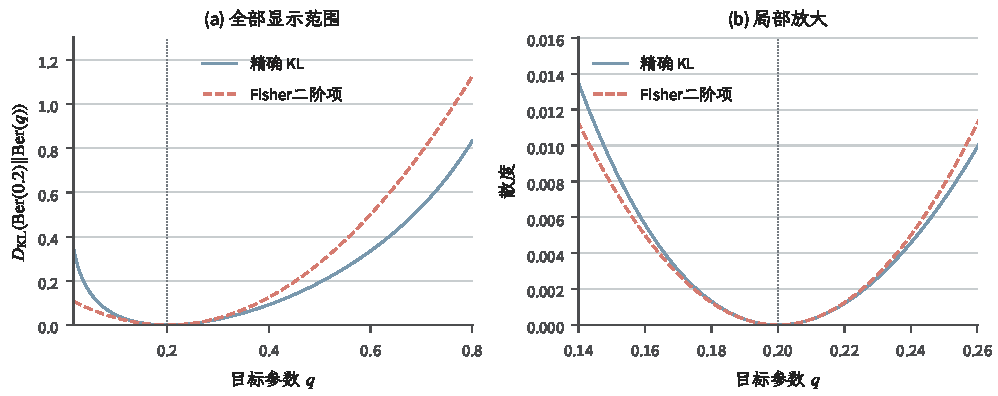
\includegraphics[width=\linewidth]{figures/01-mathematical-preliminaries/04-random-variables-distributions-and-causality/matplotlib/probability-discrete/information-fisher-local.pdf}
  \caption{Bernoulli族在\(p=0.2\)处的Fisher局部近似（解析式教学图）。
  蓝实线为\(D_{\mathrm{KL}}(P_{0.2}\Vert P_q)\)，红虚线为
  \((q-0.2)^2/[2(0.2)(0.8)]\)；右图放大邻域。图中\(0<q<1\)，
  二阶式只描述足够小的参数扰动。}
  \label{fig:information-fisher-local}
\end{figure*}

\paragraph{重参数化下的几何保持}
\label{sec:information-fisher-reparameterization}

令\(\bm\theta=\bm\theta(\bm\phi)\)为光滑局部可逆坐标变换，
Jacobian为\(\bm J=\partial\bm\theta/\partial\bm\phi\)。
在对应点\(P_{\bm\phi}=P_{\bm\theta(\bm\phi)}\)是同一张分布，
不是又施加一次统计扰动。链式法则给出
\[
  \bm s_{\bm\phi}=\bm J^\top\bm s_{\bm\theta},\qquad
  \bm F_{\bm\phi}=\bm J^\top\bm F_{\bm\theta}\bm J.
\]
因切向量满足\(\mathrm d\bm\theta=\bm J\,\mathrm d\bm\phi\)，
\[
  \mathrm d\bm\phi^\top\bm F_{\bm\phi}\mathrm d\bm\phi
  =\mathrm d\bm\theta^\top\bm F_{\bm\theta}\mathrm d\bm\theta.
\]
对同一标量目标\(L\)，梯度坐标变为
\(\bm g_{\bm\phi}=\bm J^\top\bm g_{\bm\theta}\)，
因此目标微分
\(\bm g_{\bm\phi}^\top\mathrm d\bm\phi
=\bm g_{\bm\theta}^\top\mathrm d\bm\theta\)也不变。
Fisher矩阵的数值会变，不变的是它作用于对应切向量所得到的二次型。

例如Bernoulli概率\(p\)改用logit坐标\(\phi=\log[p/(1-p)]\)，
\(\mathrm dp/\mathrm d\phi=p(1-p)\)，于是
\[
  F_\phi=\{p(1-p)\}^2F_p=p(1-p).
\]
一个坐标下的Fisher在边界附近变大，另一个变小，
但对同一分布扰动，
\((\mathrm dp)^2/[p(1-p)]=p(1-p)(\mathrm d\phi)^2\)。
坐标变换退化时不在上述局部可逆范围，例如立方高斯例子在零点的Jacobian为零。

在序贯模型中，先选对概率对象，比求逆更重要。
固定状态\(s\)，策略\(\pi_{\bm\theta}(a\mid s)\)的单步Fisher为
\[
  \bm F_s(\bm\theta)
  =\mathbb E_{A\sim\pi_{\bm\theta}(\cdot\mid s)}
    [\bm s_{\bm\theta}(s,A)\bm s_{\bm\theta}(s,A)^\top].
\]
若状态访问权重\(d(s)\)被指定并保持固定，
平均矩阵为\(\bm F_d=\mathbb E_{S\sim d}\bm F_S\)。
它衡量这一输入权重下的条件策略变化。
若把\(d_{\bm\theta}(s)\pi_{\bm\theta}(a\mid s)\)作为完整联合模型求导，
得分还包含\(\nabla\log d_{\bm\theta}(s)\)。
在正则条件下，条件策略得分均值为零，交叉项消失，联合Fisher成为
\[
  \bm F_{d_{\bm\theta}\pi_{\bm\theta}}
  =\bm F_{d_{\bm\theta}}^{\mathrm{state}}
    +\mathbb E_{d_{\bm\theta}}\bm F_S.
\]
它与把当前访问权重固定后得到的平均矩阵不是同一个对象。

第三个对象是完整轨迹Fisher。设初始分布和环境转移都不依赖参数，
参数只出现在固定有限时域\(T\)的条件动作核中。
假设共同支持和交换微分成立，各步得分二阶可积。
轨迹得分为\(\sum_{t=1}^T\bm s_t\)，其中
\(\mathbb E[\bm s_t\mid H_t]=\bm0\)，\(H_t\)为选择动作前的历史。
当\(u<t\)时，\(\bm s_u\)对\(H_t\)可测，因此
\[
  \mathbb E[\bm s_u\bm s_t^\top]
  =\mathbb E[\bm s_u\,\mathbb E(\bm s_t^\top\mid H_t)]=\bm0.
\]
展开外积便得到
\[
  \bm F_{\mathrm{trajectory}}
  =\sum_{t=1}^T\mathbb E[\bm F_{H_t}],
\]
而不是某个任意固定访问分布下的单步矩阵。
Markov策略下可把条件矩阵写成\(\bm F_{S_t}\)；
若访问权重取各时刻边缘的平均，轨迹矩阵等于对应平均矩阵的\(T\)倍。
环境或初始规律也含参数时，必须加入它们的得分，不能沿用策略独占参数的公式。

另一个常见混淆发生在样本矩阵与模型期望之间。
固定输入分布\(d\)，取条件高斯
\(Y\mid\bm X=\bm x\sim\mathcal N(\bm\theta^\top\bm x,\sigma^2)\)，
其中\(\sigma>0\)已知，\(\mathbb E_d\|\bm X\|^2<\infty\)。
同一观测的三个量为
\[
\begin{aligned}
  \bm s_{\bm\theta}(\bm x,y)
    &=\frac{y-\bm\theta^\top\bm x}{\sigma^2}\bm x,\\
  -\nabla^2_{\bm\theta}\log p_{\bm\theta}(y\mid\bm x)
    &=\frac{\bm x\bm x^\top}{\sigma^2},\\
  \bm s_{\bm\theta}\bm s_{\bm\theta}^\top
    &=\frac{(y-\bm\theta^\top\bm x)^2}{\sigma^4}\bm x\bm x^\top.
\end{aligned}
\]
按当前模型的条件分布平均时，残差平方期望为\(\sigma^2\)，
后两个矩阵的条件期望相同，再按\(d\)平均得到
\(\bm F=\mathbb E_d[\bm X\bm X^\top]/\sigma^2\)。
对一条样本，它们并不相等；残差为零时，得分外积甚至为零，
而非零输入的观测Hessian不为零。
如果真实响应规律不同于当前模型，残差平方的条件期望也可能不同，
经验得分外积的总体极限便不一定等于这个模型Fisher。
改变输入权重、使用观测Hessian或经验得分外积，都须重新说明正在近似哪个对象。

\subsubsection{局部度量下的几何更新}
\label{sec:information-geometric-update}

有了局部长度和目标微分，就可以确定在给定分布变化预算内怎样下降。
这仍是原优化任务的局部求解步骤：若参数表示有约束，应在相应可行切空间中求解，
或结合约束优化和回缩；Fisher矩阵本身不会自动保持矩与固定边缘。

\paragraph{分布变化约束下的自然梯度}
\label{sec:information-natural-gradient-update}

设目标\(L(\bm\theta)\)可微，\(\bm g=\nabla L(\bm\theta)\)，
且\(\bm F(\bm\theta)\)正定。欧氏梯度是目标微分在欧氏内积下的代表；
改用Fisher内积，代表向量也应随之改变\scite{math-amari1998natural}
\begin{definition}[自然梯度]
\label{def:information-natural-gradient}
目标\(L\)的\term{自然梯度}（natural gradient）是满足
\[
  g_{\bm\theta}(\operatorname{grad}^{F}L,\bm v)
  =\nabla L(\bm\theta)^\top\bm v
  \quad\text{对所有切向量 }\bm v
\]
的唯一向量，即
\(\operatorname{grad}^{F}L=\bm F(\bm\theta)^{-1}\nabla L(\bm\theta)\)。
\end{definition}

把目标一阶线性化，把分布KL变化二阶近似，得到局部信赖域子问题
\begin{equation}
  \min_{\bm\delta}\bm g^\top\bm\delta
  \quad\text{s.t.}\quad
  \tfrac12\bm\delta^\top\bm F(\bm\theta)\bm\delta\leq\varepsilon.
  \label{eq:information-natural-gradient-trust-region}
\end{equation}
设\(\varepsilon>0,\bm g\neq\bm0\)。
Lagrangian为
\(\bm g^\top\bm\delta+\lambda(\bm\delta^\top\bm F\bm\delta/2-\varepsilon)\)，
驻点条件给出
\(\bm g+\lambda\bm F\bm\delta=\bm0\)。
非零线性目标的最小值在椭球边界，
代入\(\bm\delta=-\lambda^{-1}\bm F^{-1}\bm g\)得到
\(\lambda=\sqrt{\bm g^\top\bm F^{-1}\bm g/(2\varepsilon)}\)，所以
\begin{equation}
  \bm\delta^\star
  =-\sqrt{\frac{2\varepsilon}{\bm g^\top\bm F^{-1}\bm g}}\,
    \bm F^{-1}\bm g.
  \label{eq:information-natural-gradient-step}
\end{equation}

可以不依赖驻点必要条件，直接验证全局最优性。
令\(\bm u=\bm F^{1/2}\bm\delta\)，约束变为
\(\|\bm u\|_2\leq\sqrt{2\varepsilon}\)，目标变为
\((\bm F^{-1/2}\bm g)^\top\bm u\)。
Cauchy--Schwarz给出
\[
  (\bm F^{-1/2}\bm g)^\top\bm u
  \geq-\|\bm F^{-1/2}\bm g\|_2\sqrt{2\varepsilon}.
\]
等号在\(\bm u\)与\(-\bm F^{-1/2}\bm g\)同向并位于球面时达到，
代回正好得到上述解。若\(\bm g=\bm0\)，一阶目标处处为零，
子问题不再选出唯一方向，应考察高阶信息或停止条件。

\begin{example}[同一分布变化预算下的两个下降方向]
\label{ex:information-natural-gradient-ellipse}
设在当前参数点，局部Fisher矩阵与目标梯度为
\[
 \bm F=\begin{pmatrix}100&0\\0&1\end{pmatrix},
 \qquad \bm g=\begin{pmatrix}1\\1\end{pmatrix}.
\]
目标的一阶变化为\(\delta_1+\delta_2\)，但同样大小的第一维位移消耗的二次KL预算
是第二维的\(100\)倍。取局部预算\(\varepsilon=0.005\)，可行椭圆为
\(100\delta_1^2+\delta_2^2\leq0.01\)。普通欧氏下降方向是\(-\bm g\)，
自然下降方向是\(-\bm F^{-1}\bm g=-(0.01,1)^\top\)。
为公平比较，把两个方向都缩放到同一椭圆边界，得到
\[
 \bm\delta_{\mathrm E}=-\frac{0.1}{\sqrt{101}}(1,1)^\top,
 \qquad
 \bm\delta_{\mathrm F}=-\frac{0.1}{\sqrt{1.01}}(0.01,1)^\top.
\]
两者都恰好消耗\(0.005\)的二次预算，目标的一阶下降量分别为
\[
 -\bm g^\top\bm\delta_{\mathrm E}
 =\frac{0.2}{\sqrt{101}}\approx0.0199,
 \qquad
 -\bm g^\top\bm\delta_{\mathrm F}
 =0.1\sqrt{1.01}\approx0.1005.
\]
自然方向减少昂贵的第一维移动，把更多预算用于第二维，因此在当前局部模型中获得
更大的下降量。这里\(\bm F\)刻画分布变化的局部代价，不是一般目标\(L\)的Hessian；
上述数值比较的是线性化目标与二次KL模型，不能直接当作真实目标的有限步下降保证。
\end{example}

图~\ref{fig:information-natural-gradient-ellipse}把两个缩放后的方向放在同一预算边界上。
两轴采用相同的物理尺度，细长椭圆说明第一维允许的位移更小。
\begin{figure}[htbp]
  \centering
  % Teaching example: F=diag(100,1), g=(1,1), epsilon=0.005.
% Both axes use 240 mm per parameter unit; the ellipse semiaxes are 0.01,0.1.
% The equal-budget endpoints are computed from the formulas in the text.
% Keep the narrow ellipse and annotate from its sides; blue/dashed/circle denotes
% Euclidean descent, red/solid/square denotes natural descent.
\begin{tikzpicture}[
  x=1mm,y=1mm,
  every node/.style={font=\figurefont\footnotesize,text=FigureInk,inner sep=1pt},
  >={Latex[length=1.5mm,width=1.1mm]}
]
  \path[use as bounding box] (0,0) rectangle (112,66);
  \coordinate (O) at (52,34);
  \coordinate (E) at ({52-24/sqrt(101)},{34-24/sqrt(101)});
  \coordinate (F) at ({52-0.24/sqrt(1.01)},{34-24/sqrt(1.01)});

  \fill[FigurePaper] (O) ellipse [x radius=2.4mm,y radius=24mm];
  \draw[FigureMuted,line width=.8pt] (O) ellipse [x radius=2.4mm,y radius=24mm];
  \draw[->,FigureStroke,line width=.6pt] (26,34)--(77,34) node[right] {\(\delta_1\)};
  \draw[->,FigureStroke,line width=.6pt] (52,6)--(52,62) node[above] {\(\delta_2\)};
  \draw[FigureStroke,line width=.6pt] (51,58)--(53,58);
  \draw[FigureStroke,line width=.6pt] (51,10)--(53,10);
  \node[anchor=west] at (56,58) {\(0.1\)};
  \node[anchor=west] at (56,7) {\(-0.1\)};
  \node[anchor=south west] at (54,35) {\(0\)};
  \node[anchor=east] at (45,49) {\(\delta_1=\pm0.01\)};
  \draw[FigureMuted,line width=.5pt] (45,46)--(49.6,34);

  \draw[->,FigureBlue,dashed,line width=1pt] (O)--(E);
  \fill[FigureBlue] (E) circle (.7mm);
  \draw[FigureBlue,line width=.6pt] (E)--(36,26)--(22,26);
  \node[anchor=east,text=FigureBlue] at (34,22) {欧氏方向\(\bm\delta_{\mathrm E}\)};

  \draw[->,FigureRed,line width=1pt] (O)--(F);
  \fill[FigureRed] ($(F)+(-.7,-.7)$) rectangle ($(F)+(.7,.7)$);
  \draw[FigureRed,line width=.6pt] (F)--(66,16);
  \node[anchor=west,text=FigureRed] at (68,16) {自然方向\(\bm\delta_{\mathrm F}\)};
\end{tikzpicture}

  \caption{局部KL预算下的下降方向（解析式教学图）。灰色椭圆满足
  \(100\delta_1^2+\delta_2^2=0.01\)，对应\(\varepsilon=0.005\)。
  蓝色虚线与圆点是缩放后的欧氏方向\(\bm\delta_{\mathrm E}\)，红色实线与方点是
  自然方向\(\bm\delta_{\mathrm F}\)；两个终点消耗相同的二次预算。
  椭圆表达分布变化代价，不是目标函数的等高线。}
  \label{fig:information-natural-gradient-ellipse}
\end{figure}

在光滑可逆重参数化下，由上一小节的矩阵和微分变换，
\[
\begin{aligned}
  \bm J\bm F_{\bm\phi}^{-1}\bm g_{\bm\phi}
  &=\bm J(\bm J^\top\bm F_{\bm\theta}\bm J)^{-1}
    \bm J^\top\bm g_{\bm\theta}\\
  &=\bm F_{\bm\theta}^{-1}\bm g_{\bm\theta}.
\end{aligned}
\]
归一化因子中的
\(\bm g_{\bm\phi}^\top\bm F_{\bm\phi}^{-1}\bm g_{\bm\phi}\)
也等于原坐标下的相应值，因此两个坐标给出同一个分布切向方向。
Bernoulli例子中，自然梯度在概率坐标为\(p(1-p)L'(p)\)，
在logit坐标为\(L'(p)\)；乘上\(\mathrm dp/\mathrm d\phi=p(1-p)\)后相同。

保持的是无穷小方向，不是任意有限离散步。
非线性坐标映射下，
\(\bm\theta(\bm\phi+\bm\delta_\phi)
=\bm\theta(\bm\phi)+\bm J\bm\delta_\phi+O(\|\bm\delta_\phi\|^2)\)，
所以分别做欧氏加法更新后的终点一般不同。
真实KL也还有\(o(\|\bm\delta\|^2)\)余项；
二次预算等于\(\varepsilon\)不保证真实KL严格不超过它。
有限步需要步长选择、真实目标或KL检查，不能由局部方向不变性直接得到全局改进。

\paragraph{奇异与近似条件下的几何更新}
\label{sec:information-singular-approximate-update}

参数冗余、退化坐标或不足的输入方向都可能使Fisher奇异。
其零空间只说明相应方向的一阶得分为零：
有时它来自完全冗余，有时如立方高斯零点，只是高阶变化未被二次型看见。
因而不能把所有零方向都理解成有限移动后分布完全不变。

回用伪逆与数值求解工具，若\(\bm g\in\operatorname{range}(\bm F)\)，
线性方程\(\bm F\bm v=\bm g\)有解，全部解为
\[
  \bm v=\bm F^\dagger\bm g+\bm z,\qquad
  \bm z\in\ker\bm F.
\]
伪逆选择当前欧氏坐标下范数最小的一个。
在得分能识别的切向商空间中，零空间分量不影响一阶分布方向，
但参数向量并不唯一，有限步的高阶效果仍可能不同。
若\(\bm g\notin\operatorname{range}(\bm F)\)，存在零方向
\(\bm z\)使\(\bm g^\top\bm z\neq0\)；
沿其下降方向任意放大仍不消耗二次预算，线性信赖域问题无下界。
此时简单写\(\bm F^\dagger\bm g\)不是原信赖域子问题的解，必须修正退化模型或约束。

阻尼使用\(\bm F+\lambda\bm I\)，其中\(\lambda>0\)，可改善病态性并保证可逆。
但它新增欧氏二次项\(\lambda\|\bm\delta\|^2\)，不是纯粹的Fisher几何：
一般坐标变化下
\[
  \bm J^\top(\bm F+\lambda\bm I)\bm J
  =\bm J^\top\bm F\bm J+\lambda\bm J^\top\bm J
  \neq\bm F_{\bm\phi}+\lambda\bm I.
\]
因此“能稳定求逆”与“保持原坐标变换性质”是不同要求。
实际计算通常求解线性系统，而不显式构造逆矩阵；
迭代容差、谱条件和矩阵近似误差也会改变得到的方向。

经验Fisher、分块或对角近似可能降低计算量，
却分别引入抽样、模型期望或跨块相关性的近似。
即使每个近似矩阵都正定，也只说明定义了某种局部内积，
不说明它等于真实分布Fisher，更不保证同样的坐标保持结论。
应区分模型下期望、真实数据下平均、固定输入权重和完整轨迹，
再说明哪一项被估计或省略。
优化收敛、模型正确性、预测校准和隐私保证还各有自己的条件；
自然梯度或KL正则不能把一种保证自动转成另一种。

\section{本章小结}
\label{sec:information-theory-statistical-geometry-summary}

开篇的编码与预测问题对应两个不同对象。
熵平均单个结果的自信息，条件熵记录已有观测后还需描述的部分；
交叉熵把预测规律放到真实规律下评价，多出的对数代价是有方向的KL。
互信息则比较联合分布与独立乘积，带噪二元例子显示观测究竟减少了多少不确定性。
连续情形必须指定参考测度，微分熵的坐标变化不能与KL的坐标不变性混为一谈。

比较两张分布时，要先说明希望看见什么差别。
总变差看到事件概率，MMD看到所选核函数类，Wasserstein看到质量移动的距离；
R\'enyi通过密度比高阶矩控制权重迁移。相同均值可以掩盖分布差异，
点质量的小位移可以保持平滑评价稳定，却使阈值事件完全改变。
因此小距离只有结合取值范围、敏感性或尾部条件，才能变成具体任务保证。
数据选择还要另付依赖代价：互信息控制平均有符号偏差，
PAC--Bayes在固定先验和参数下控制同时风险。

信息不足也给出反向限制。Le Cam与Fano要求同时构造目标分离、观测接近的候选，
自适应观测则沿实际历史累计条件信息，不能当作固定设计的独立样本。
这些结论限制任何算法能够知道什么，不等于某个算法已经达到下界。

分布优化又把比较量变成目标或约束。
Gibbs倾斜权衡收益和KL偏离，最大熵从给定矩中选择相容分布，
ELBO在表示受限的候选族中逼近后验；固定边缘的搬运问题只选择联合配对。
有限配置的负最大熵与配分函数共轭在边界仍成立，
但分布最优解不一定有有限参数表示。
最优耦合依赖紧性与成本下半连续，后验逼近依赖明确方向的支持条件。

参数化求解时，正则满秩模型的局部KL给出Fisher度量，
自然梯度据此选择同一分布切向方向。
奇异性、阻尼、矩阵近似与有限步余项都限制这一结论的直接使用。
局部几何不能替代全域散度，优化替代分布也不能替代真实数据证据。
若问题从观测规律转为干预会怎样改变结果，还需要
第~\ref{chap:causal-inference}章的生成机制与识别条件。
